\documentclass[journal,onecolumn]{IEEEtran}
\usepackage{cite}
\renewcommand{\citepunct}{,}
\usepackage{amssymb}
\usepackage{amsmath}
\usepackage{epsfig}
\usepackage{graphicx}
\usepackage{amsfonts}
\usepackage{colortbl}
\usepackage{multirow}
\usepackage{booktabs}
\usepackage{longtable}
\usepackage{array}
\usepackage{bm}
\usepackage{multicol}
\usepackage{algorithmic}
\usepackage{amsthm}
\usepackage[linesnumbered,ruled,vlined]{algorithm2e}
\usepackage{mathtools}
\usepackage[dvipsnames,table]{xcolor}
\usepackage{subfigure}
\usepackage{paralist}
\usepackage{color}
\DeclareMathOperator{\dir}{dir}
\usepackage{tabu}
\usepackage{rotating}
\usepackage{pifont}
\usepackage{threeparttable}
\usepackage{moresize}
\usepackage{cancel}
\usepackage{pgf-pie}
\usepackage{adjustbox}
\usepackage{url}
\usepackage{makecell}
\usepackage{float}
\usepackage{placeins}
\usepackage{setspace}
\usepackage{enumitem}
\usepackage{comment}
\usepackage{epstopdf}
\usepackage{booktabs,multirow}
\usepackage{pdflscape}
\usepackage{titlesec}
\usepackage[hidelinks]{hyperref}
\usepackage[mathlines,switch]{lineno}

\graphicspath{{../Figs_manual/}{Figs_manual/}}

\newcommand{\CM}{\ding{51}}
\newcommand{\XM}{\ding{53}}
\newcolumntype{L}{>{\raggedleft}p{0.14\textwidth}}
\newcolumntype{R}{p{0.8\textwidth}}
\newcommand\VRule{\color{lightgray}\vrule width 0.5pt}
\DeclareMathOperator{\sign}{sgn}

\def\hl{\setlength{\fboxsep}{1.0pt}\colorbox[rgb]{0.85,0.85,0.85}}

\newtheorem{example}{Example}
\newtheorem*{example*}{Example}
\newtheorem{definition}{Definition}
\newtheorem{theorem}{Theorem}
\newtheorem{lemma}{Lemma}
\newtheorem{proposition}{Proposition}

\newcommand{\argmin}[1]{\underset{#1}{\operatorname{arg\ min}}}
\renewcommand{\vec}{\mathbf}
\newcommand{\manualfigwidth}{0.92\linewidth}
\setlength{\extrarowheight}{2pt}
\setlength{\emergencystretch}{1em}
\setcounter{secnumdepth}{3}

% Manual-specific numbering.
\renewcommand*{\thesection}{\arabic{section}}
\renewcommand*{\thesubsection}{\thesection.\arabic{subsection}}
\renewcommand*{\thesubsubsection}{\thesubsection.\arabic{subsubsection}}
\renewcommand*{\thetable}{\arabic{table}}
\renewcommand*{\thefigure}{\arabic{figure}}
\renewcommand*{\theequation}{\arabic{equation}}
\makeatletter
\makeatother

\titleformat{\section}
  {\normalfont\large\bfseries\raggedright}
  {\thesection}{0.75em}{}
\titleformat{\subsection}
  {\normalfont\normalsize\bfseries\raggedright}
  {\thesubsection}{0.75em}{}
\titleformat{\subsubsection}
  {\normalfont\normalsize\itshape\raggedright}
  {\thesubsubsection}{0.75em}{}
\titlespacing*{\section}{0pt}{2.0ex plus 0.5ex minus 0.2ex}{1.0ex}
\titlespacing*{\subsection}{0pt}{1.5ex plus 0.4ex minus 0.2ex}{0.8ex}
\titlespacing*{\subsubsection}{0pt}{1.2ex plus 0.3ex minus 0.2ex}{0.6ex}

\title{PORTAL Studio: Research Workflow User Guide}
\author{PORTAL Contributors}

\begin{document}
\maketitle
\begin{quote}
\small
This guide covers recipe construction, experiments, and visual exploration in the Python version of PORTAL Studio. It can be read and built independently of the companion manuscripts. The public PORTAL preprint~\cite{portal2025framework} provides the framework background; reusable curation and augmentation workflows are documented in the accompanying repository.
\end{quote}
\tableofcontents
\clearpage

\section{Installation and First Launch}
\label{sec:manual:installation}

Use Python 3.11 or newer in a dedicated environment. From the repository root,
run \texttt{python -m venv .venv}. Activate it in Windows PowerShell with:
\begin{verbatim}
.\.venv\Scripts\Activate.ps1
\end{verbatim}
On macOS or Linux, use \texttt{source .venv/bin/activate} instead. Then run:
\begin{verbatim}
python -m pip install -r requirements.txt
python -m pip check
python -m portal_studio.gui.app
\end{verbatim}
The standard installation uses PySide6 and includes the native optimizers and
the PuLP/CBC dependency for curation. To install optional NiaPy and pymoo algorithms:
\begin{verbatim}
python -m pip install -r requirements-algorithms.txt
\end{verbatim}
PyTorch acceleration is optional; the NumPy evaluator does not require it.
No MATLAB or R installation is needed. The repository README summarizes the
tested environment.

The public distribution contains code and recipe JSONs, not the papers' raw
feature tables, optimizer results, or experimental realizations. Studio and
the runners create new results in user-controlled output directories. Use a
writable checkout and start with a small FE budget.

\section{The PORTAL Framework}
\label{sec:manual:conceptual}

PORTAL is a framework for constructing continuous black-box optimisation problems with controllable landscape structure. Users assemble problems with selected basin geometry, conditioning, variable interaction, ruggedness, multimodality, and block-wise composition.

The framework background is described in the public preprint~\cite{portal2025framework}. This guide explains the operations available in Studio's three workspaces and identifies the separate suite-construction and augmentation runners where relevant.

PORTAL problems are constructed through three layers:

\begin{itemize}
\item \textbf{Layer~1 -- Component.} A component is the basic basin-forming object. It defines its centre, mathematical formulation, curvature, conditioning, orientation, objective-value offset, and optional transformations.

\item \textbf{Layer~2 -- Landscape.} One or more components of the same dimension are combined into a landscape. When multiple components are used, the lower-envelope construction creates competing component basins across the search space.

\item \textbf{Layer~3 -- Block-wise composition.} Landscapes defined over different variable blocks are combined through weighted contributions to form the complete objective function. Multiple blocks allow partial separability and heterogeneous structures or contribution strengths across variable groups.
\end{itemize}

Table~\ref{tab:manual:key-terms} summarises the main PORTAL terms used throughout this guide.

\begin{table}[H]
\centering
\small
\caption{Core PORTAL terms used in this guide.}
\label{tab:manual:key-terms}

\begin{tabular}{@{}p{0.22\linewidth}p{0.68\linewidth}@{}}
\toprule
\textbf{Term} & \textbf{Meaning in the workflow} \\
\midrule

\textbf{Recipe} &
A complete, reproducible PORTAL structural and parameter specification. \\

\textbf{Component} &
The Layer~1 basin-forming object, with its own formulation, centre, shape controls, orientation, objective-value offset, and optional transformations. \\

\textbf{Landscape} &
A Layer~2 function formed from one or more components of the same dimension. With multiple components, the lower-envelope construction creates competing component basins. \\

\textbf{Block} &
A subset of decision variables with its own landscape and contribution weight in the Layer~3 composition. \\

\textbf{Realisation} &
A mode-specific use or controlled derivation of a source recipe for evaluation. \\

\textbf{Instance} &
The concrete objective landscape defined by the resulting specification and used for inspection, analysis, or optimisation. \\

\bottomrule
\end{tabular}
\end{table}

PORTAL uses minimisation: components compete within a block, and positively weighted block landscapes are added over disjoint variable sets. This separates the blocks additively; interactions can remain within each block, including those created by component competition.

The known optimum requires valid component parameters and minimising centres inside the evaluation domain. Components can have additional minimisers, and competition can hide individual basins. Studio assigns each variable to one block, allowing all blocks to attain their minima simultaneously. If blocks shared variables, their minimising values could conflict.

\section{PORTAL Studio Workflow Overview}
\label{sec:manual:studio-provides}

PORTAL Studio is organised around three connected workspaces:

\begin{itemize}
\item \textbf{Generator:} authors PORTAL recipes and prepares concrete instances for analysis or evaluation. Users can inspect generated parameters, perform Exploratory Landscape Analysis (ELA), save instances as PORTAL JSON files, or select prepared instances in the Experiment workspace.

\item \textbf{Experiment:} evaluates optimisers on PORTAL instances under reproducible run settings. It accepts instances prepared in Generator or loaded from PORTAL JSON files, supports built-in and user-added optimisers, and records repeated-run results for convergence analysis, final absolute error summaries, and statistical comparison.

\item \textbf{Education:} provides interactive two-dimensional authoring, visualisation, and optimiser demonstrations. Users can edit component parameters directly, inspect components and complete landscapes, compare configurations side by side, and evaluate built-in or user-added optimisers.
\end{itemize}

For research workflows, problems are typically constructed and characterised in Generator and then evaluated in Experiment. Education provides a complementary two-dimensional environment for visual exploration, teaching, demonstration, and controlled comparison of landscape configurations.

To start Studio, install the repository requirements in the configured project environment and run the following from the repository root:
\begin{quote}\ttfamily
python -m portal\_studio.gui.app
\end{quote}
The GUI uses PySide6; the active environment determines the available numerical and optional solver packages. Keep the saved instance, software revision, package versions, solver settings, budgets, and seeds with research results.

For automated benchmark curation and train/test construction, use
\path{run_suite_pipeline.py}. It performs measurement, feature preparation,
de-duplication, selection, and JSON materialization. Its configuration and split
controls are documented in \path{Recipe_Selection/suite_pipeline/README.md}.
The separate \path{run_augmentation_dataset.py} runner creates Type~3 JSONs
without running ELA or optimizers; see
\path{Recipe_Selection/augmentation_pipeline/README.md}.

\paragraph{First-use walkthrough.}
The following route produces a saved problem, an ELA export, and optimisation results; the later sections explain each setting.
\begin{enumerate}
\item In \emph{Generator}, select \emph{+ Add Block}. Use the block-row plus control to open a new component, configure its parameters, and select \emph{+ Add Component}.
\item Select \emph{Prepare Instance for ELA}, then \emph{Save Instance JSON} to preserve the concrete problem.
\item In the ELA panel, tick the prepared instance, choose the sample factor and feature groups, and select \emph{Run ELA}. Choose the Excel output file when prompted.
\item Open \emph{Experiment}: the instance prepared in Generator automatically appears in the \emph{Problem instance} list. Select it, or use \emph{Load Instance} to load a saved JSON file. Choose \emph{Source}, \emph{Algorithm}, algorithm parameters, run count, FE budget, seed policy, and realisation type. Select \emph{+ Add Task}.
\item Tick the task in \emph{Pending Tasks}, choose the pool and workers, and select \emph{Run Selected Tasks}.
\item Check the terminal state and error summaries in \emph{Finished Tasks}. Select the completed task in \emph{Statistical Analysis} for \emph{Trend Plots} or \emph{Box Plots}; statistical tests require multiple compatible completed tasks.
\end{enumerate}

\subsection{Data and File Operations}
\label{ssec:manual:data-operations}

PORTAL Studio supports several forms of inspection, modification, persistence, and export across the three workspaces. Table~\ref{tab:manual:data-operations} summarises their roles.

\begin{table}[H]
\centering
\small
\caption{Data operations and file roles in PORTAL Studio.}
\label{tab:manual:data-operations}
\begin{tabular}{@{}p{0.24\linewidth}p{0.66\linewidth}@{}}
\toprule
\textbf{Operation group} & \textbf{Role in the workflow} \\
\midrule
\textbf{Inspection} & Generated-parameter tables, rotation tables, ELA outputs, finished-task summaries, statistical-test tables, convergence plots, and box plots expose values produced during construction and evaluation. \\
\textbf{Modification} & Reroll and seeded-reroll actions resample generated values; copy controls reuse compatible realised values; clone creates an independently editable component duplicate. \\
\textbf{Persistence} & PORTAL JSON files store concrete benchmark problems. Finished-result ZIP archives preserve task settings, run errors, convergence data, and analysis identities for later import. SQLite result bundles store the underlying measurements. \\
\textbf{Analysis and export} & ELA feature tables can be exported to Excel; Statistical Analysis plots can be exported as PNG, PDF, or SVG; Education plots can be saved as PDF. \\
\bottomrule
\end{tabular}
\end{table}

Keep the instance JSON for later problem evaluation. To reopen completed experiments for analysis in a later session, export and import finished-result archives as described in Section~\ref{ssec:manual:experimental-task-execution}.

\subsection{Using Help in the Interface}
\label{ssec:manual:interface-help}

PORTAL Studio provides contextual help throughout the interface. The question-mark \emph{Help} button in the toolbar starts a guided tour of the main workspaces (Figure~\ref{fig:manual:interface-help}), while nearby question-mark controls explain individual parameters, tables, and settings.

\begin{figure}[H]
    \centering
    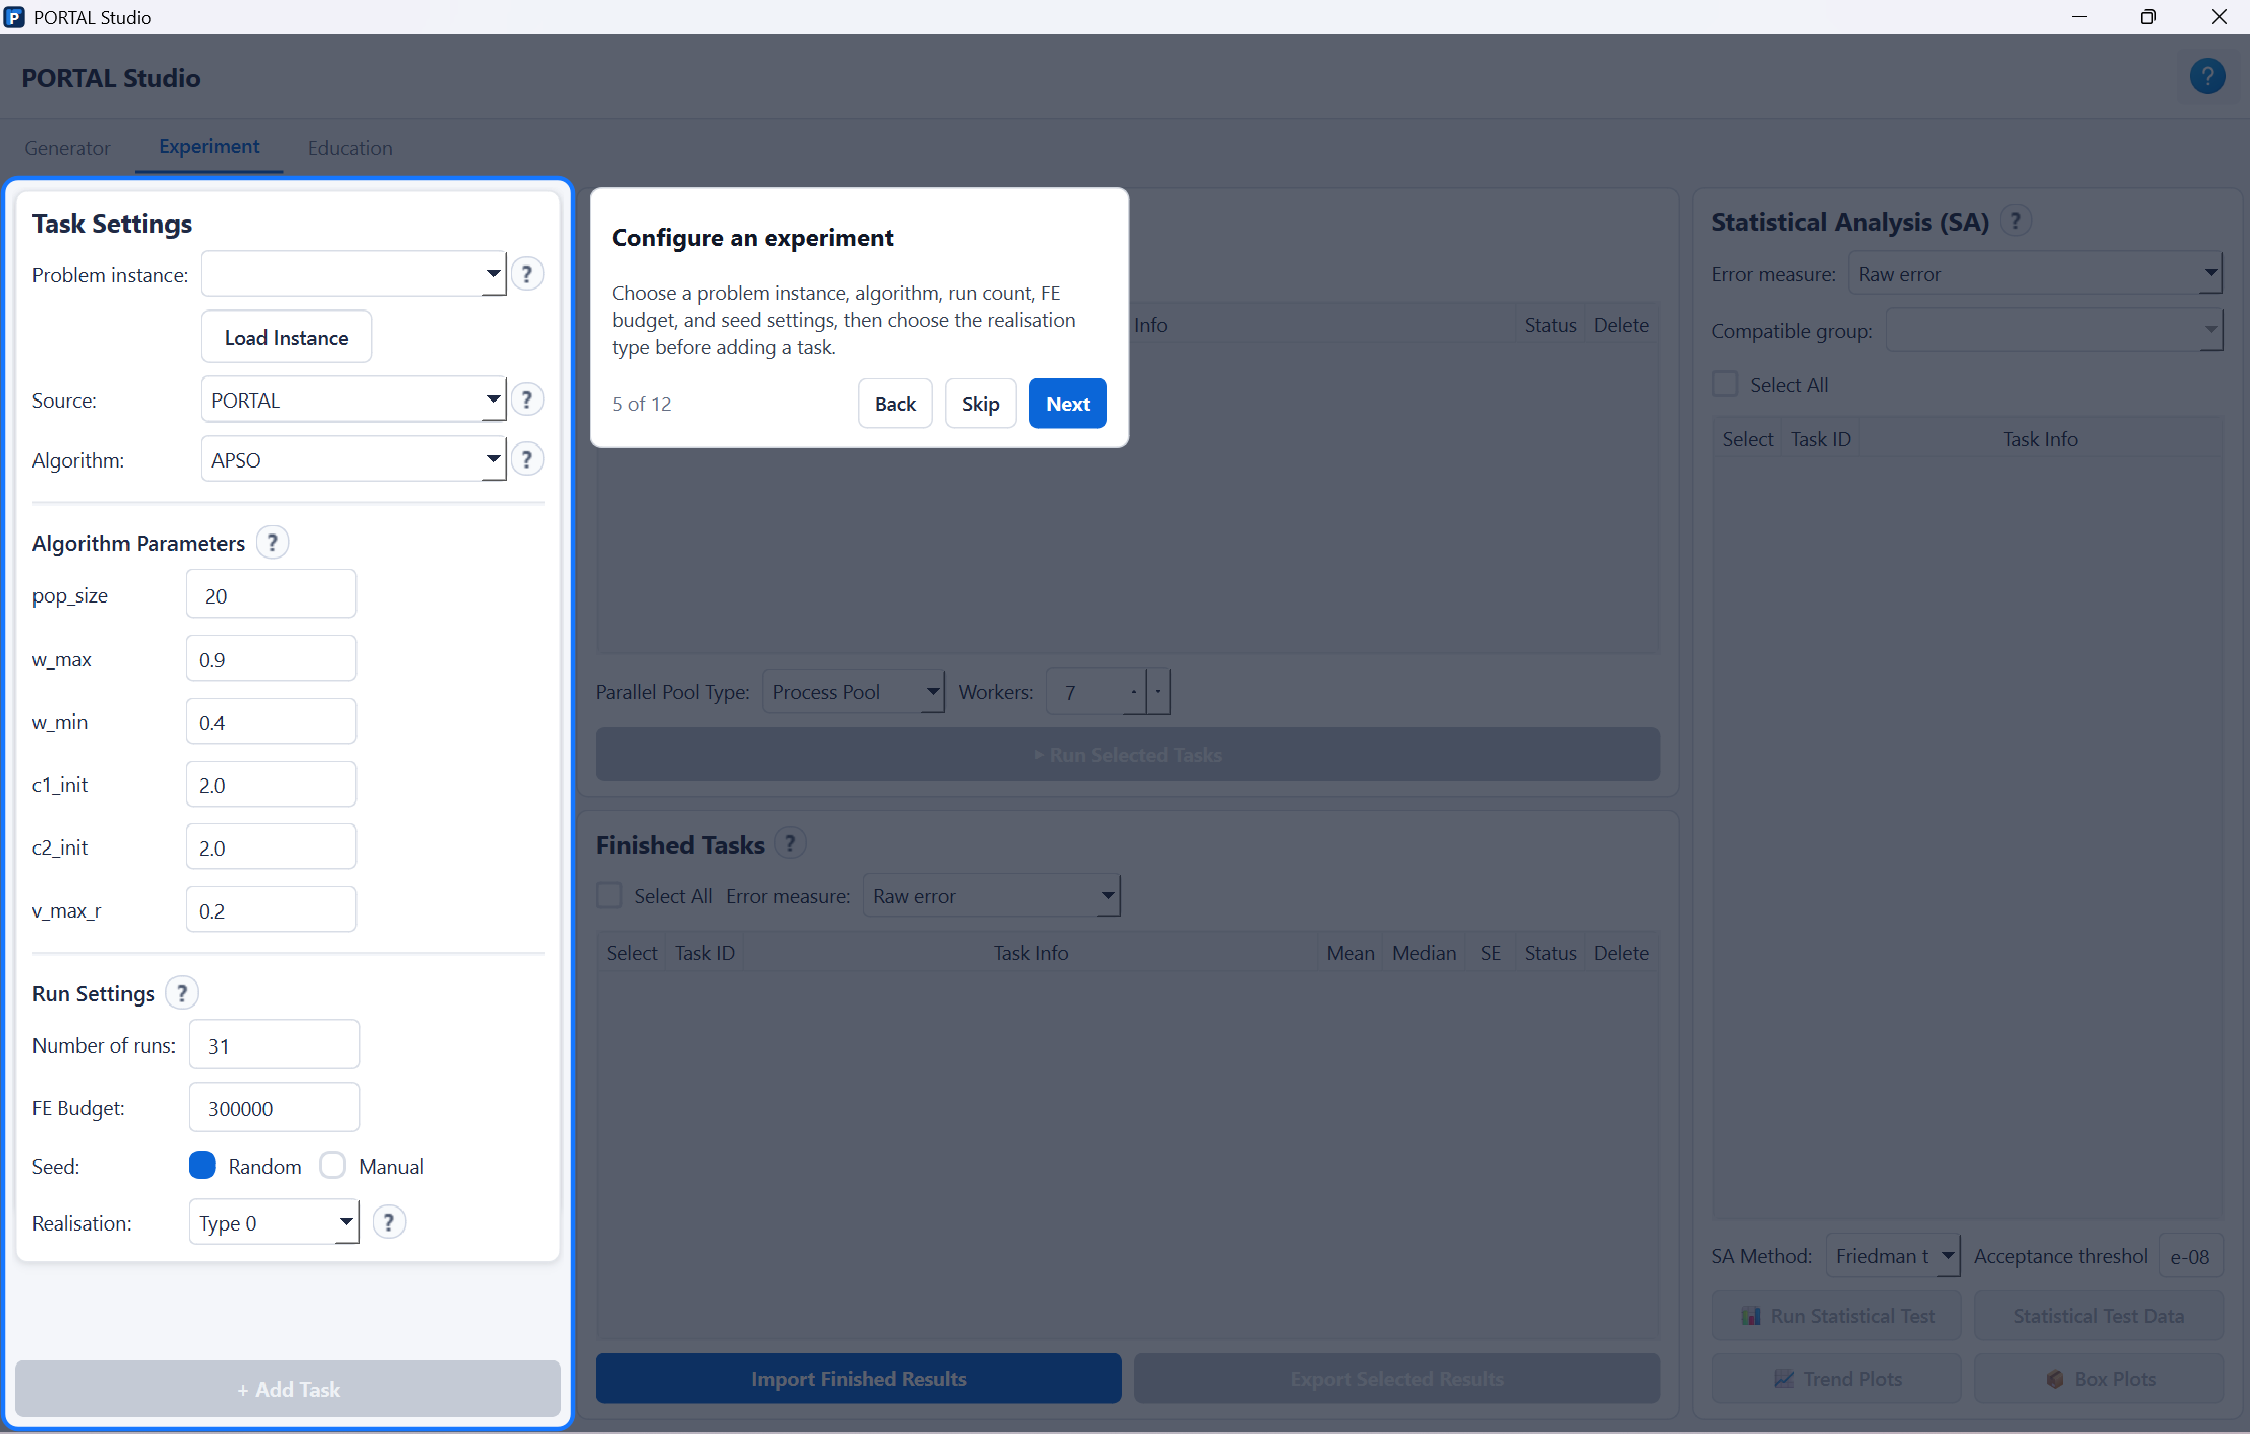
\includegraphics[width=\manualfigwidth]{10.png}
    \caption{Guided tour highlighting Task Settings in Experiment. The guide explains the selected panel and provides Back, Skip, and Next controls.}
    \label{fig:manual:interface-help}
\end{figure}

\section{Generator Workspace}
\label{sec:manual:generator}

The Generator workspace is the main authoring environment for constructing PORTAL recipes and preparing concrete instances for analysis. As shown in Figure~\ref{fig:manual:generator-workspace}, it contains three panels: the left panel defines the block/component hierarchy, the middle panel edits the selected block or component, and the right panel analyses prepared instances using ELA.

\begin{figure}[!t]
    \centering
    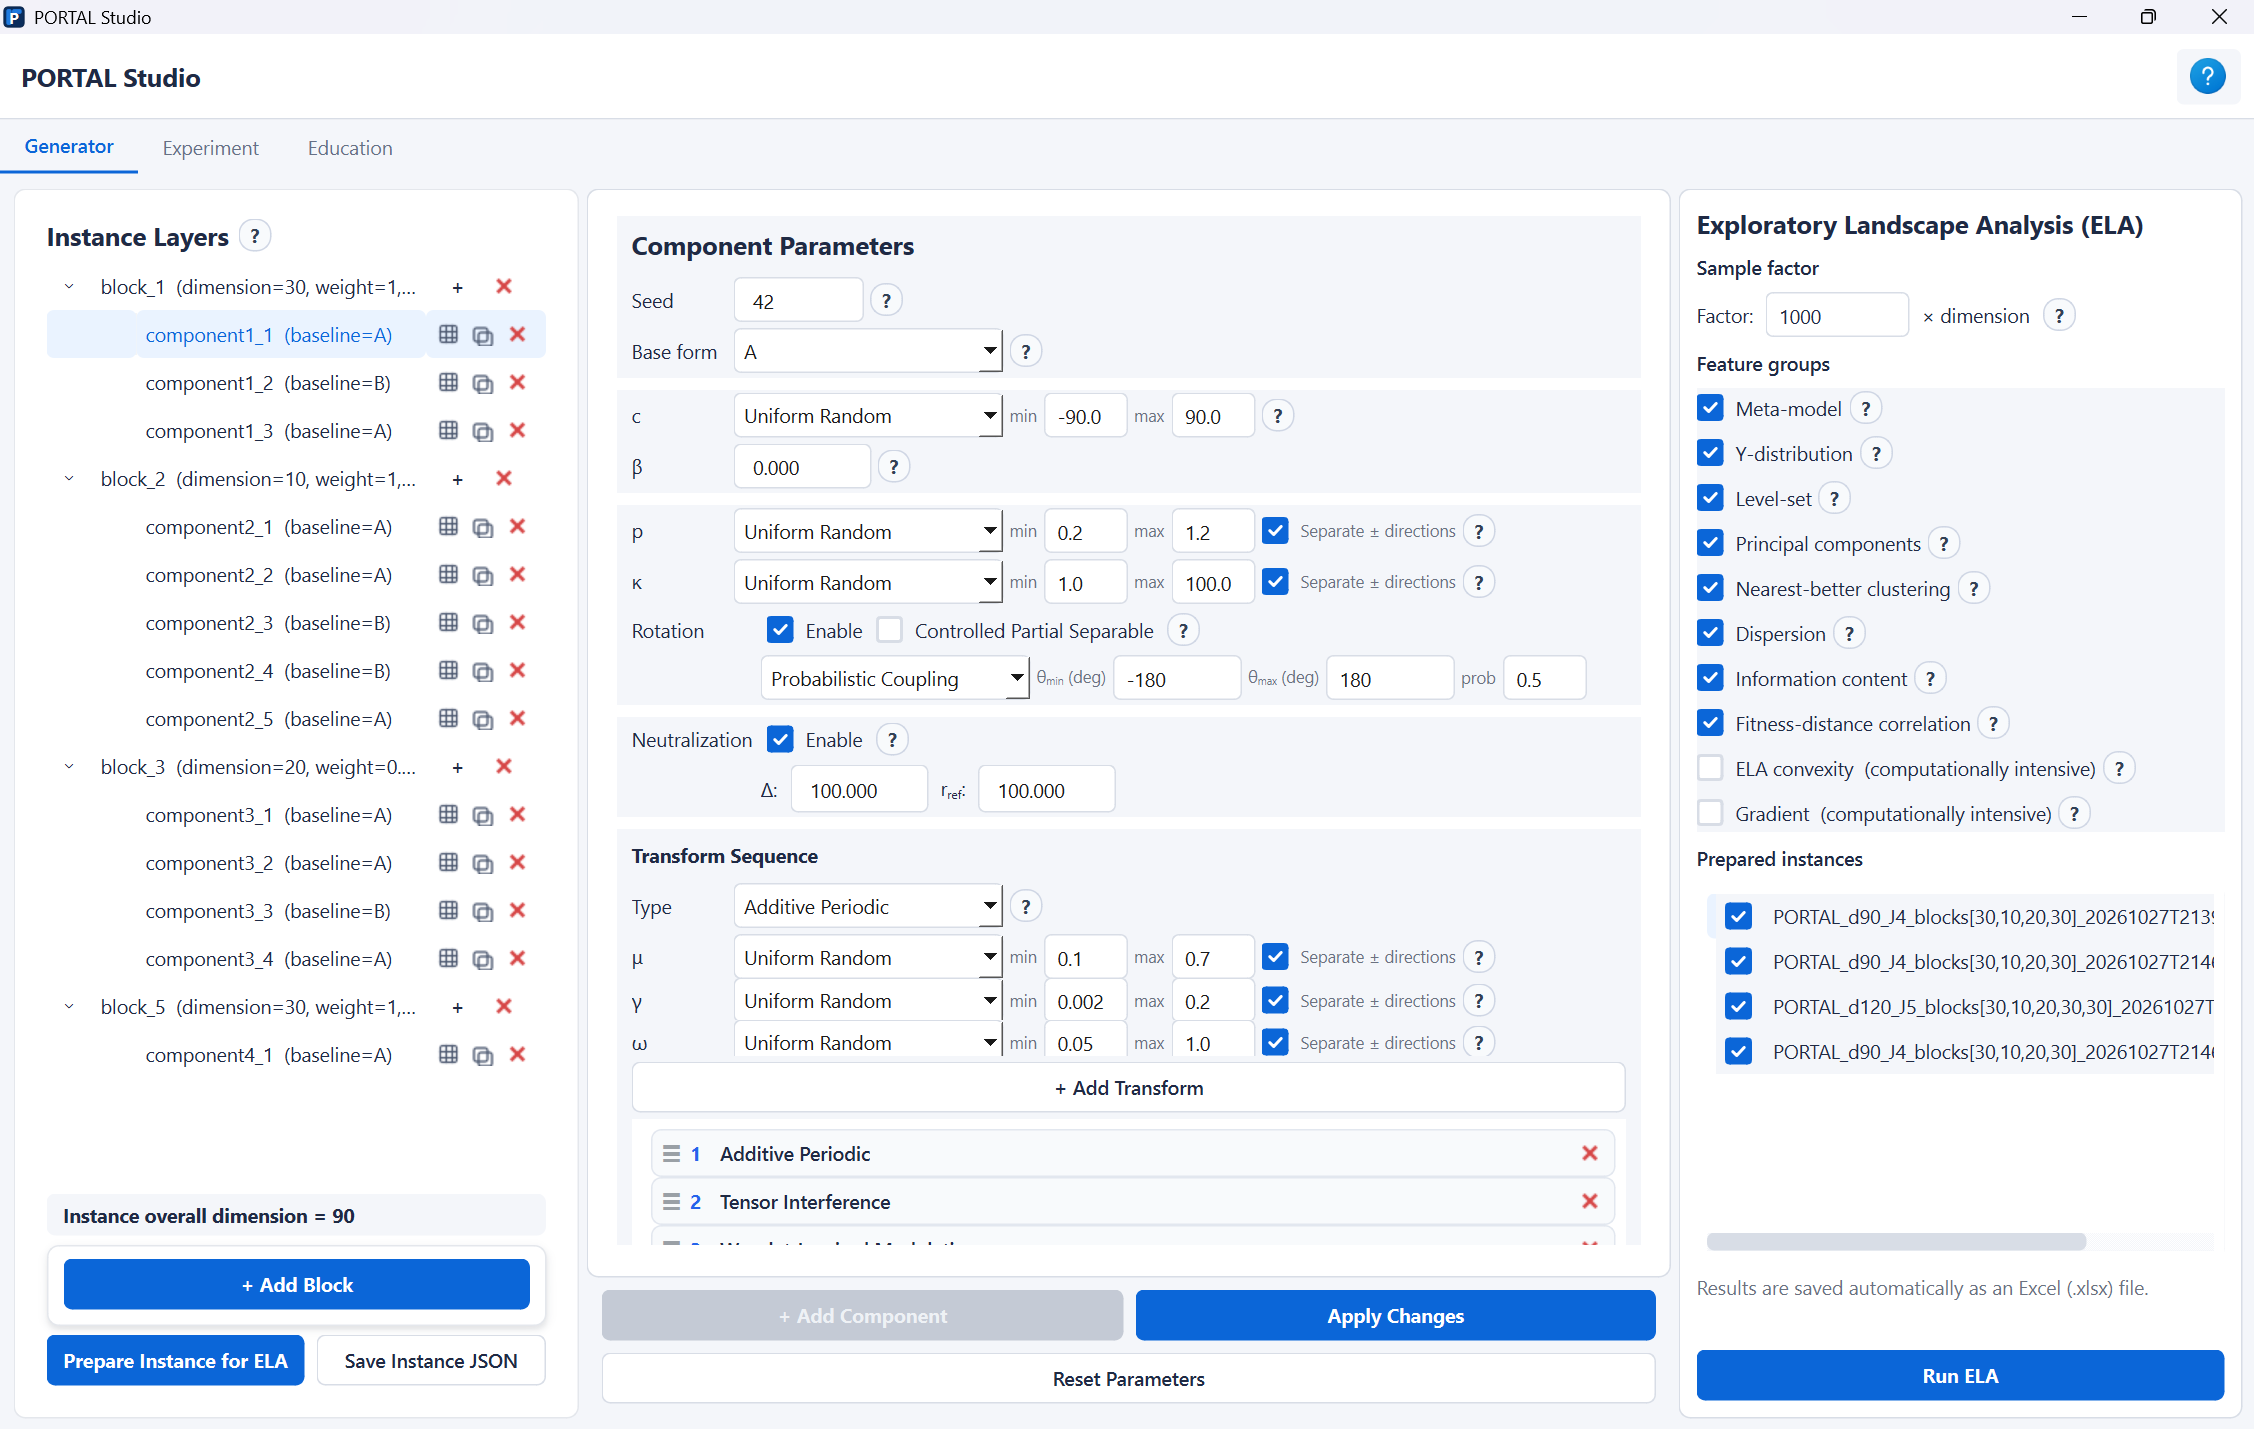
\includegraphics[width=\manualfigwidth]{1.png}
    \caption{Generator workspace with the block/component hierarchy on the left, component settings in the middle, and exploratory landscape analysis on the right. Question-mark controls provide contextual help.}
    \label{fig:manual:generator-workspace}
\end{figure}

\subsection{Instance Layers}
\label{ssec:manual:generator-authoring}

The \emph{Instance Layers} panel represents the current recipe as a block-and-component tree. Select \emph{+ Add Block} to create a block, initially with dimension 30 and weight 1. Each block must have at least two dimensions, as specified in Part~I.

Select a block to edit its dimension and weight in the middle panel's \emph{Block Parameters}, then commit with \emph{Apply Changes}. Changing a populated block's dimension prompts for confirmation and regenerates all component values, including rotations and transformations, from the stored generation specifications and effective random streams. Existing coordinates are regenerated rather than simply extended. Inspect the new values and prepare a new instance after applying the change.

Use the plus control on a block row to open a new component editor. Configure the fields in \emph{Component Parameters}, then select \emph{+ Add Component} to store it in that block. To edit an existing component, select its tree row, change the fields, and select \emph{Apply Changes}. Components within a block share its dimension and combine through the lower-envelope construction. Component-row controls open generated parameters, clone the component, or delete it.

\subsection{Component Parameters}
\label{ssec:manual:generator-parameters}

The \emph{Component Parameters} panel defines the selected Layer~1 component. Choose its base form, location, shape, rotation, and optional transformations, then commit the settings as described above.

The \emph{Base form} selector chooses between PORTAL's two component formulations. \emph{Base Form A} corresponds to the per-direction exponent formulation (Form~1 in Part~I), while \emph{Base Form B} corresponds to the shared single-exponent formulation (Form~2).

For either formulation, users can configure the component's centre, curvature, anisotropy, objective-value offset, rotation, and transformations. Each setting is briefly described below; the framework preprint~\cite{portal2025framework} gives the mathematical construction.

The exponent \(p\) controls basin curvature and growth away from the component centre. The setting \(p=1\) gives the quadratic reference case; values below and above 1 produce subquadratic and superquadratic growth, respectively. The linear-growth reference is $p=0.5$; lower values give sublinear growth and higher values give superlinear growth.

The anisotropy factors \(\kappa\) control directional scaling. Equal \(\kappa\) values give equal directional scaling, while a higher ratio of the largest to the smallest factor produces greater directional contrast. Even with equal anisotropy factors, unequal curvature exponents can produce different growth profiles across directions.

For component \(k\), Base Form A assigns separate curvature exponents \(p^+_{k,i}\) and \(p^-_{k,i}\) to the positive and negative sides of each coordinate \(i\). Base Form B uses one exponent \(p_k\) for the entire component, while retaining directional anisotropy through \(\kappa^\pm_{k,i}\).

The centre \(c\) controls the component location in the search space, while the vertical offset \(\beta\) sets its objective value at that centre. Within a multi-component block, the components compete through the lower-envelope construction. In a multi-block instance, the block-level landscapes are combined using their contribution weights.

Enable \emph{Neutralization} to reduce unintended scale differences when changing curvature or anisotropy. Set $r_{\mathrm{ref}}$ as the reference displacement along each coordinate and $\Delta$ as the target reference rise above the component's centre value. This calibration preserves directional differences.

After changing curvature exponents, anisotropy factors, or the block dimension, apply the edits and prepare a new instance. Studio automatically recalculates the calibration factors $\rho$ when \emph{Neutralization} is enabled; otherwise, it sets them to one. The interface retains the label \emph{Neutralization} for this calibration control.

Rotation sets the orientation of the component's internal coordinate system through pairwise angles. Leave \emph{Enable} unchecked for \emph{No Rotation}. Otherwise, enable rotation and choose a mode from the dropdown, or tick \emph{Controlled Partial Separable} and select \emph{Configure}. All angle inputs and rotation tables use degrees. Table~\ref{tab:manual:rotation-modes} summarises the modes.

\begin{table}[H]
\centering
\small
\caption{Rotation modes available in the Generator workspace.}
\label{tab:manual:rotation-modes}
\begin{tabular}{@{}p{0.28\linewidth}p{0.62\linewidth}@{}}
\toprule
\textbf{Mode} & \textbf{Interpretation} \\
\midrule
\textbf{No Rotation} & Sets all pairwise rotation angles to zero, leaving the component axes aligned with the coordinate axes. \\
\textbf{Fully Connected} & Assigns an angle to every variable pair, producing dense coordinate mixing. \\
\textbf{Probabilistic Coupling} & Selects each variable pair according to a user-defined probability; only selected pairs receive rotation angles. \\
\textbf{Uniform Random Angle} & Applies one sampled angle to all variable pairs. \\
\textbf{Fixed Angle} & Applies one user-specified angle to all variable pairs. \\
\textbf{Chain-like Coupling} & Specifies angles only for neighbouring coordinate pairs; combining these rotations can indirectly mix non-neighbouring coordinates. \\
\textbf{Controlled Partial Separable} & Divides variables into groups and applies rotation only within groups, leaving cross-group rotation entries zero. \\
\bottomrule
\end{tabular}
\end{table}

For \emph{Controlled Partial Separable}, the \emph{Configure} dialog (Figure~\ref{fig:manual:controlled-partial-separable}) specifies automatic or manual group sizes and the within-group angle policy. Coordinates are randomly assigned to groups of the requested sizes. Rotation mixes coordinates only within each group; any unassigned coordinates remain unchanged by the rotation. These groups control rotation only. The component formulation, transformations, and competition between components can introduce additional variable interactions.

\begin{figure}[H]
    \centering
    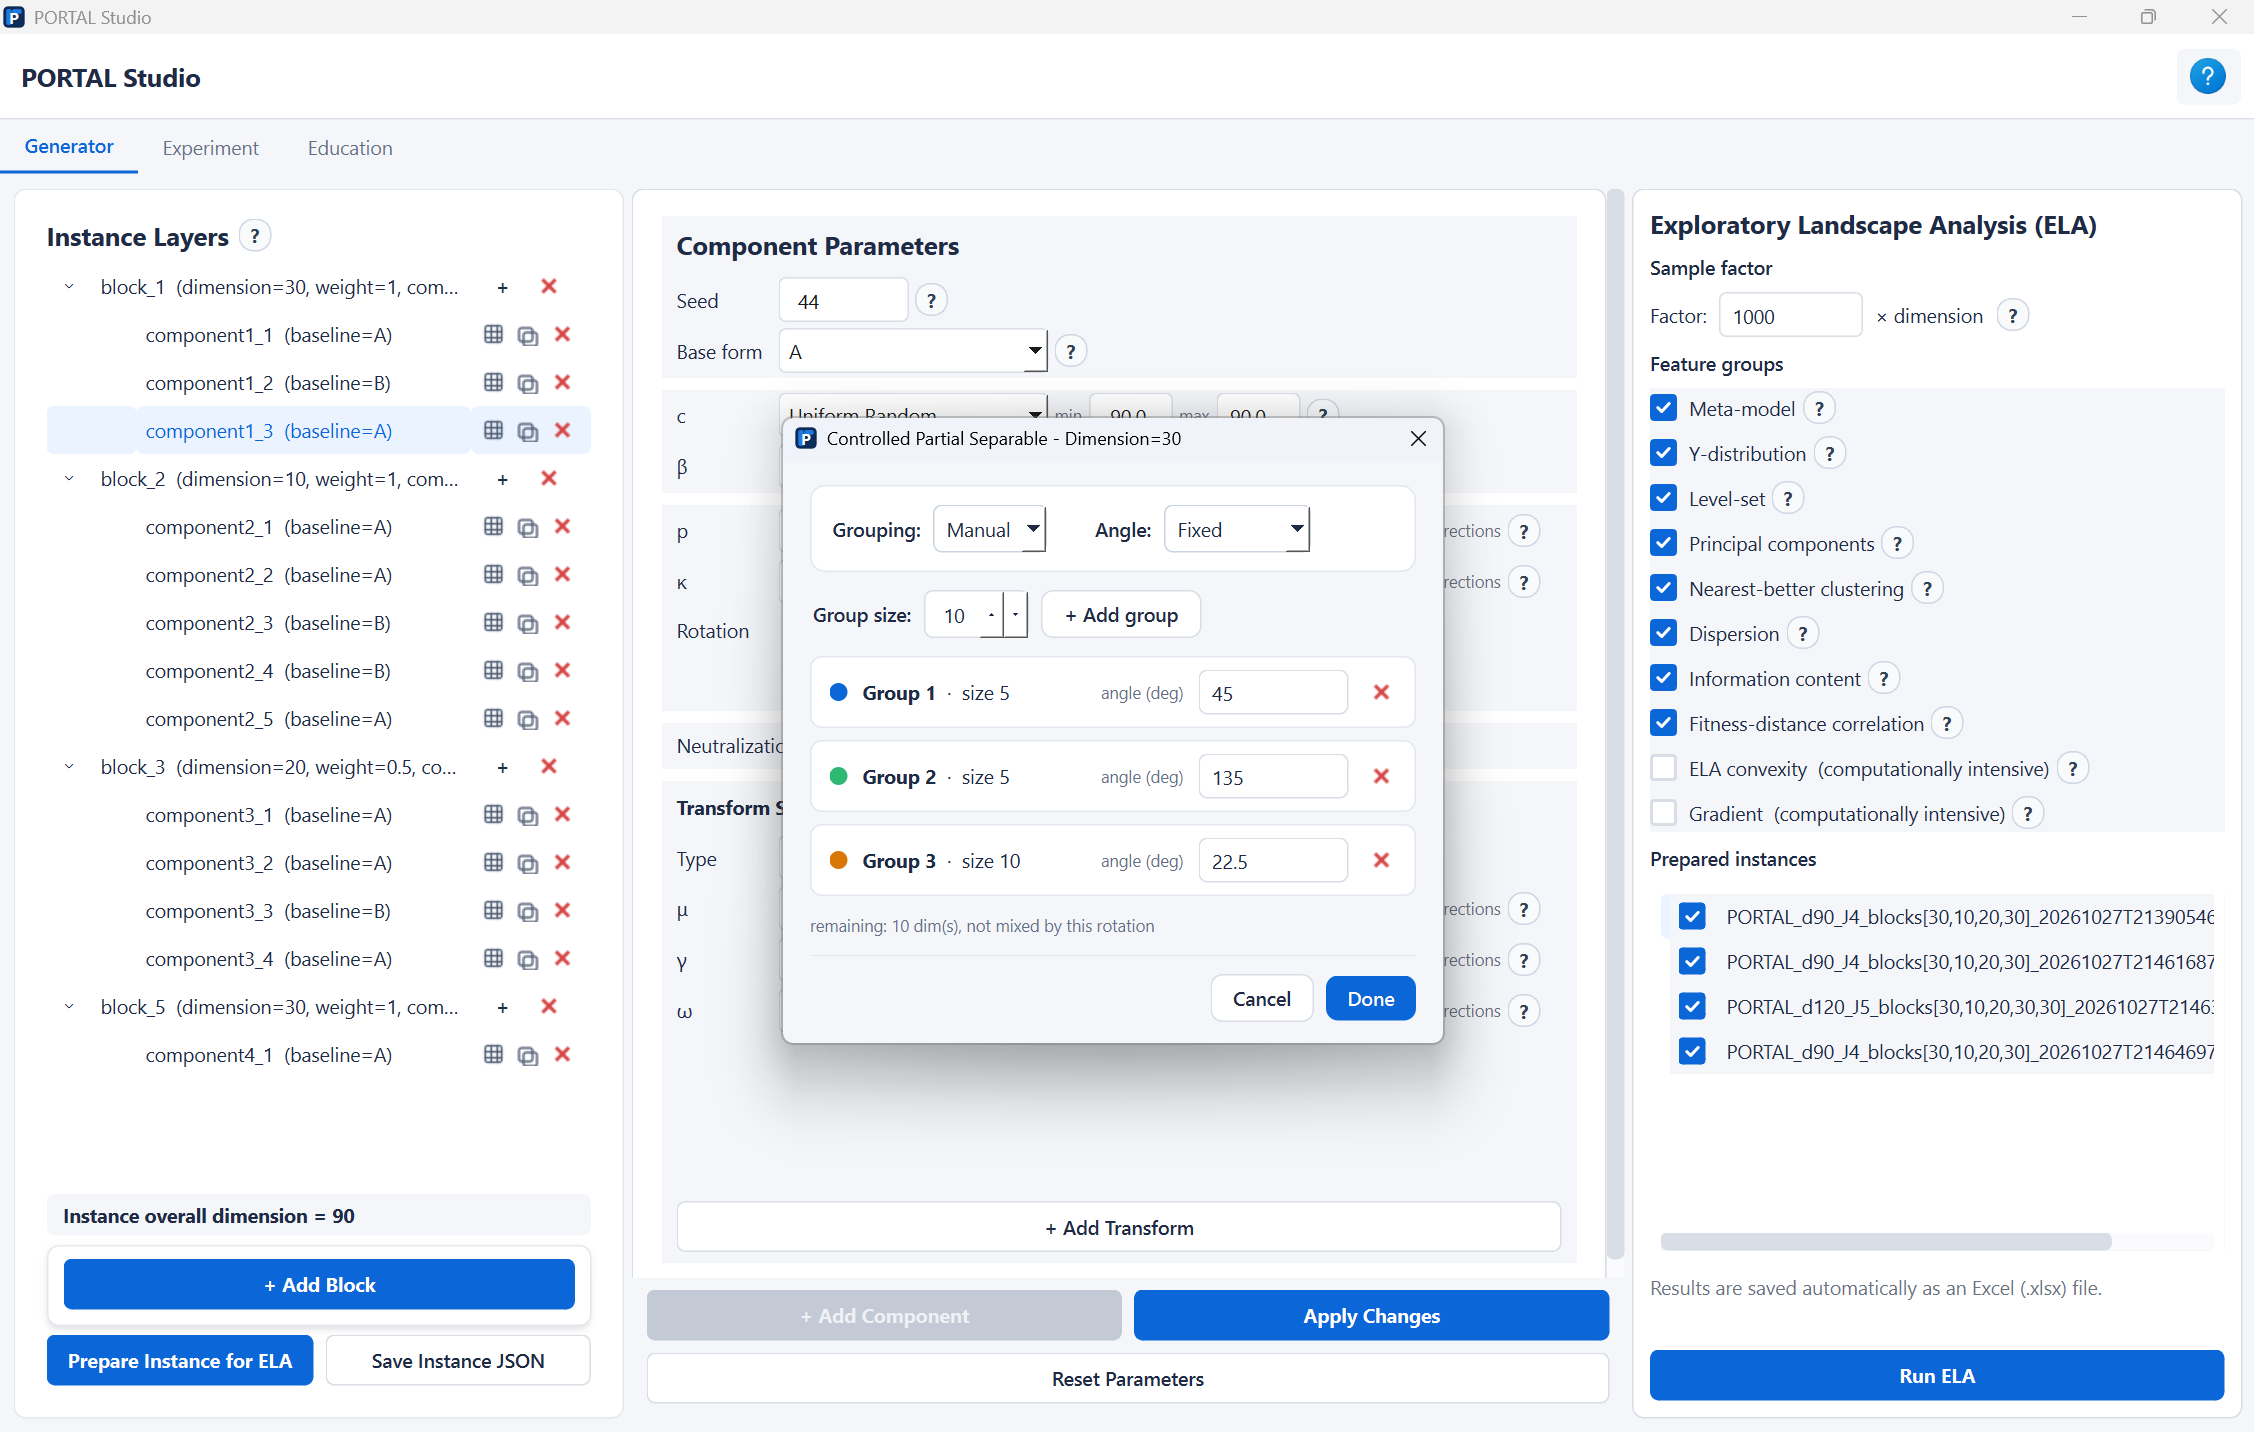
\includegraphics[width=\manualfigwidth]{5.png}
    \caption{Manual rotation grouping in a 30-dimensional component. Groups of sizes 5, 5, and 10 use fixed angles of $45^\circ$, $135^\circ$, and $22.5^\circ$, respectively; the remaining 10 dimensions are not mixed by this rotation.}
    \label{fig:manual:controlled-partial-separable}
\end{figure}

\subsubsection{Transformations}
\label{ssec:manual:generator-transformations}

Transformations add controlled ruggedness and local structure to a component. A component without transformations retains its baseline basin geometry, while transformed components can exhibit repeated oscillations, localised ruggedness, cross-coordinate interference, or radial structures.

PORTAL distinguishes element-wise and coupling transformations. Element-wise transformations act independently on each internal coordinate after rotation. Coupling transformations depend jointly on multiple internal coordinates and can introduce additional non-separability.

Multiple transformations can be applied sequentially to the same component. Their order is part of the recipe and can affect the resulting landscape. Table~\ref{tab:manual:transformation-operators} summarises the transformation operators available for component-level ruggedness control.

\begin{table}[H]
\centering
\small
\caption{Transformations available for component-level ruggedness control. Their parameters can be explored visually in the Education workspace.}
\label{tab:manual:transformation-operators}
\begin{tabular}{@{}p{0.30\linewidth}p{0.60\linewidth}@{}}
\toprule
\textbf{Transformation} & \textbf{Effect on the component} \\
\midrule
\textbf{Additive Periodic} & Adds regular coordinate-wise oscillations, producing repeated local structure. \\
\textbf{Log-Sinusoidal} & Introduces scale-sensitive oscillation in logarithmic coordinate space. \\
\textbf{Wavelet-Inspired Modulation} & Adds localised oscillations along each internal coordinate, with extent controlled by an envelope. \\
\textbf{Tensor Interference} & Introduces cross-coordinate interference and structured coupling. \\
\textbf{Radial Polynomial-Trigonometric} & Applies radial modulation based on distance from the centre, introducing concentric structure. \\
\bottomrule
\end{tabular}
\end{table}

To add a transformation in Generator, choose its \emph{Type} in the \emph{Transform Sequence} area, configure the displayed parameters, and select \emph{+ Add Transform}. Drag a sequence row to reorder it, or use its cross control to delete it. For an existing component, commit sequence changes with \emph{Apply Changes}; for a new component, use \emph{+ Add Component}. To edit an existing transformation, select its row, change the settings, and select \emph{Apply Changes}. The component stores transformations, parameters, and order together. Only transformations added to the sequence are applied.

\emph{Repeated transformation types:} Each transformation keeps its own settings and is applied in the listed order, even when the same type is used more than once.

\subsubsection{Randomisation Modes}
\label{ssec:manual:generator-randomisation}

Most Generator parameters use a generation mode together with a range or mode-specific setting. The selected mode determines how parameter values are generated across dimensions and, where applicable, across positive and negative directions (see Section~\ref{ssec:manual:generator-separate-directions}).

\begin{table}[H]
\centering
\small
\caption{Randomisation modes and their definitions. Available modes depend on the selected parameter.}
\label{tab:manual:parameter-generation-modes}
\begin{tabular}{@{}p{0.22\linewidth}>{\raggedright\arraybackslash}p{0.68\linewidth}@{}}
\toprule
\textbf{Mode} & \textbf{Definition} \\
\midrule
\textbf{Uniform Random} & Samples each coordinate value independently and uniformly from the specified range. \\
\textbf{With Exclusion Zone} & Samples centre coordinates outside an excluded interval placed inside the centre sampling range, choosing the lower or upper allowed interval with equal probability. \\
\textbf{Fixed Value} & Uses the user-specified exponent in every coordinate. \\
\textbf{Fixed Gradient} & Assigns evenly spaced exponents from the minimum to the maximum in coordinate order. \\
\textbf{Beta Distribution} & Samples values from a beta distribution mapped to the specified range. Shape parameters $\alpha,\beta>0$ give a symmetric distribution when equal; unequal values favour one end. \\
\textbf{Linear Spread (Shuffled)} & Generates evenly spaced values across the specified range and randomly permutes their coordinate assignments. \\
\textbf{Isotropic Random} & Samples one anisotropy factor and uses it for every coordinate of the component. \\
\textbf{Fixed Unit Scale \((\kappa=1)\)} & Sets every anisotropy factor to one. \\
\textbf{Dimension-shared} & Samples one value for a transformation parameter and uses it across all coordinates of the component. \\
\bottomrule
\end{tabular}
\end{table}

\subsubsection{Separate Directional Values}
\label{ssec:manual:generator-separate-directions}

Parameters with positive and negative directional forms use matched values by default: the negative-side values are copied from the corresponding positive-side values.

Where available, \emph{Separate \(\pm\) directions} generates the two signs independently from the shared generation mode and sampling bounds. This allows directional asymmetry in curvature, conditioning, or transformation strength.

\subsubsection{Clone, Reroll, Seeded Reroll, and Copy}
\label{ssec:manual:generator-parameter-actions}

Open a component's generated-parameter table using its table icon in \emph{Instance Layers}. \emph{Reroll} is shown initially; tick \emph{Seeded reroll} or \emph{Copy} above the table to reveal those action columns. The available actions are:

\begin{itemize}
\item \emph{Clone} copies a component into a selected block. The clone is independently editable and is regenerated to match the target block dimension when necessary.
\item \emph{Reroll} regenerates one parameter row using its generation mode and settings. A matched negative-side row follows a rerolled positive-side row. Rerolling a copied value (see \emph{Copy} below) removes its copy override, so it is generated independently of the source component.
\item \emph{Seeded reroll} regenerates a parameter row using a user-specified seed. The same seed reproduces the same values when applied to a compatible parameter row with the same generation settings.
\item \emph{Copy} takes a one-time snapshot of a parameter's current value from another component with the same dimension and base form. Transformation parameters additionally require the same transformation type at the same sequence position. Repeat \emph{Copy} to resynchronise after source edits; copied values do not update automatically.
\end{itemize}

Use Table~\ref{tab:manual:generator-parameter-actions} to choose an action. Figure~\ref{fig:manual:clone-component} shows the destination selection for a cloned component.

\begin{figure}[H]
    \centering
    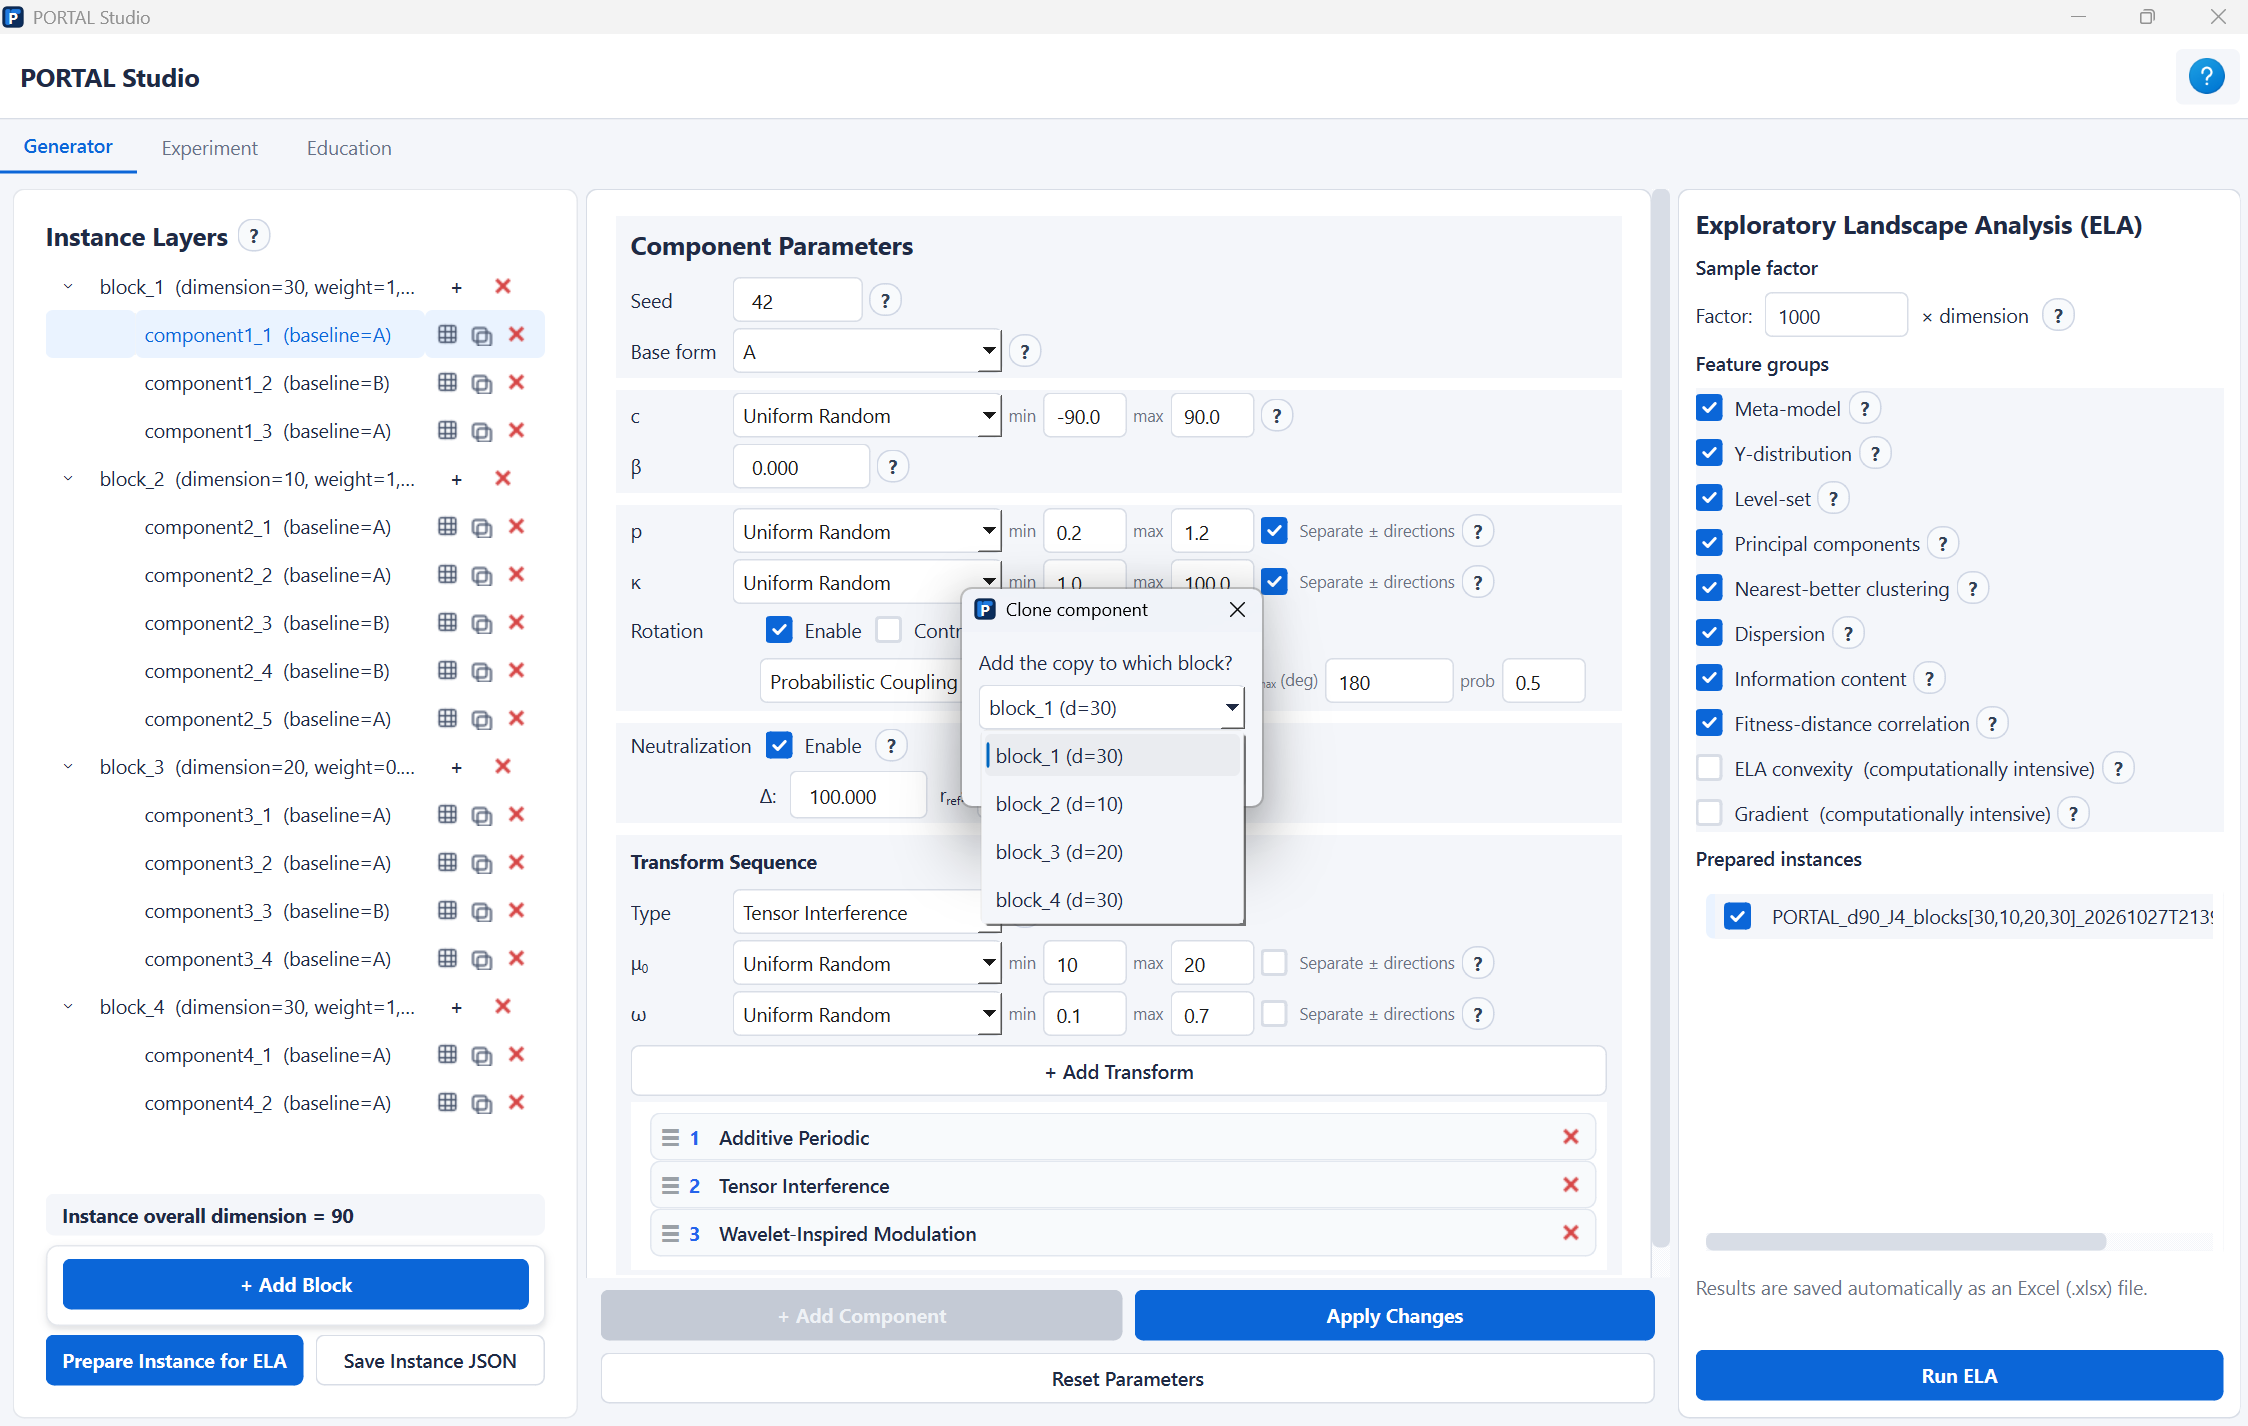
\includegraphics[width=\manualfigwidth]{4.png}
    \caption{Clone-component dialog for choosing the destination block.}
    \label{fig:manual:clone-component}
\end{figure}

\begin{table}[H]
\centering
\small
\caption{Choosing among Clone, Reroll, Seeded reroll, and Copy. Component~A has already been created. The scenarios below show how to create component~B from A, or change B after it has been created.}
\label{tab:manual:generator-parameter-actions}
\begin{tabular}{@{}p{0.35\linewidth}p{0.17\linewidth}p{0.38\linewidth}@{}}
\toprule
\textbf{What you want} & \textbf{Action} & \textbf{Result} \\
\midrule
Create B as a complete copy of A. & \textbf{Clone A} & Creates B with A's settings and values. Choose a destination block with the same dimension to retain the values. \\
Generate another centre for B using B's current sampling settings. & \textbf{Reroll B's centre} & Generates another centre without asking you to enter a seed. \\
Generate B's centre using a seed you choose. & \textbf{Seeded reroll B's centre} & Reproduces the same centre when that seed, dimension, and generation settings are reused. \\
Give B the same centre as A, keeping B's other settings. & \textbf{Copy A's centre onto B} & Copies A's current centre. Later changes to A do not update B automatically. \\
\bottomrule
\end{tabular}
\end{table}

Each parameter normally uses the component seed. \emph{Seeded reroll} assigns a separate seed to the selected parameter. To return to the component seed, open the generated-parameter table, tick \emph{Seeded reroll}, then right-click the parameter's button in the \emph{seed} column and choose \emph{Clear row seed}. This regenerates its values. Because rerolls, separate seeds, and copied parameters affect the final values, save the instance JSON with your results to preserve the exact problem evaluated.

\subsubsection{Preparing and Saving Instances}
\label{ssec:manual:generator-preparation}

Each block must contain at least one component. Apply any pending edits with \emph{Apply Changes}, then select \emph{Prepare Instance for ELA}. The prepared instance appears in the ELA panel and becomes available in Experiment without saving and reloading.

Select \emph{Save Instance JSON} and choose a filename and folder. After editing the problem, apply the changes and prepare the instance again. You can then save it under the same filename to replace the previous version, or choose a different name to keep both. To use the saved problem in a later session, select \emph{Load Instance} in Experiment and choose the JSON file.

\subsection{Exploratory Landscape Analysis}
\label{ssec:manual:generator-ela}

The Exploratory Landscape Analysis panel computes landscape features using \texttt{pflacco}~\cite{prager2024pflacco}. Select one or more prepared instances, set the sample factor, and choose the feature groups. The initial sample size is the factor multiplied by the instance dimension.

The sample factor defaults to 1000 and accepts values from 10--10,000. Sampling uses an improved Latin-hypercube design over the instance bounds with a fixed internal seed of 42. The default initial design for $d=30$ therefore contains 30,000 points.

The ten groups are meta-model, response distribution, level-set, principal components, nearest-better clustering, dispersion, information content, fitness-distance correlation, ELA convexity, and gradient. The computationally intensive convexity and gradient groups are initially unchecked; enable them for protocols that use all ten.

Select \emph{Run ELA}, confirm the export prompt, and choose an Excel output file. Studio writes the feature values when processing finishes. \emph{Stop ELA} requests cancellation; a cancelled analysis saves no ELA file. Before comparing instances, check the \texttt{failed\_groups} column to identify feature groups that could not be calculated. Leave missing results as missing values; replacing them with zero would incorrectly treat them as measured results.

ELA estimates depend on sample size, design, implementation, and seed. Use consistent settings and versions across comparisons. Exports contain raw descriptors; use the separate suite runner for preprocessing, redundancy assessment, and performance-based curation. Its feature-preparation settings are described in \path{Recipe_Selection/suite_pipeline/README.md}.


\FloatBarrier
\section{Experiment Workspace}
\label{sec:manual:experimental}

The \emph{Experiment} workspace lets users evaluate and compare optimisation algorithms on PORTAL problems. Users can configure repeated runs, examine errors and convergence, and perform statistical comparisons.

As shown in Figure~\ref{fig:manual:experimental-workspace}, the workspace is organised into \emph{Task Settings}, \emph{Pending Tasks}, \emph{Finished Tasks}, and \emph{Statistical Analysis}.

\begin{figure}[H]
    \centering
    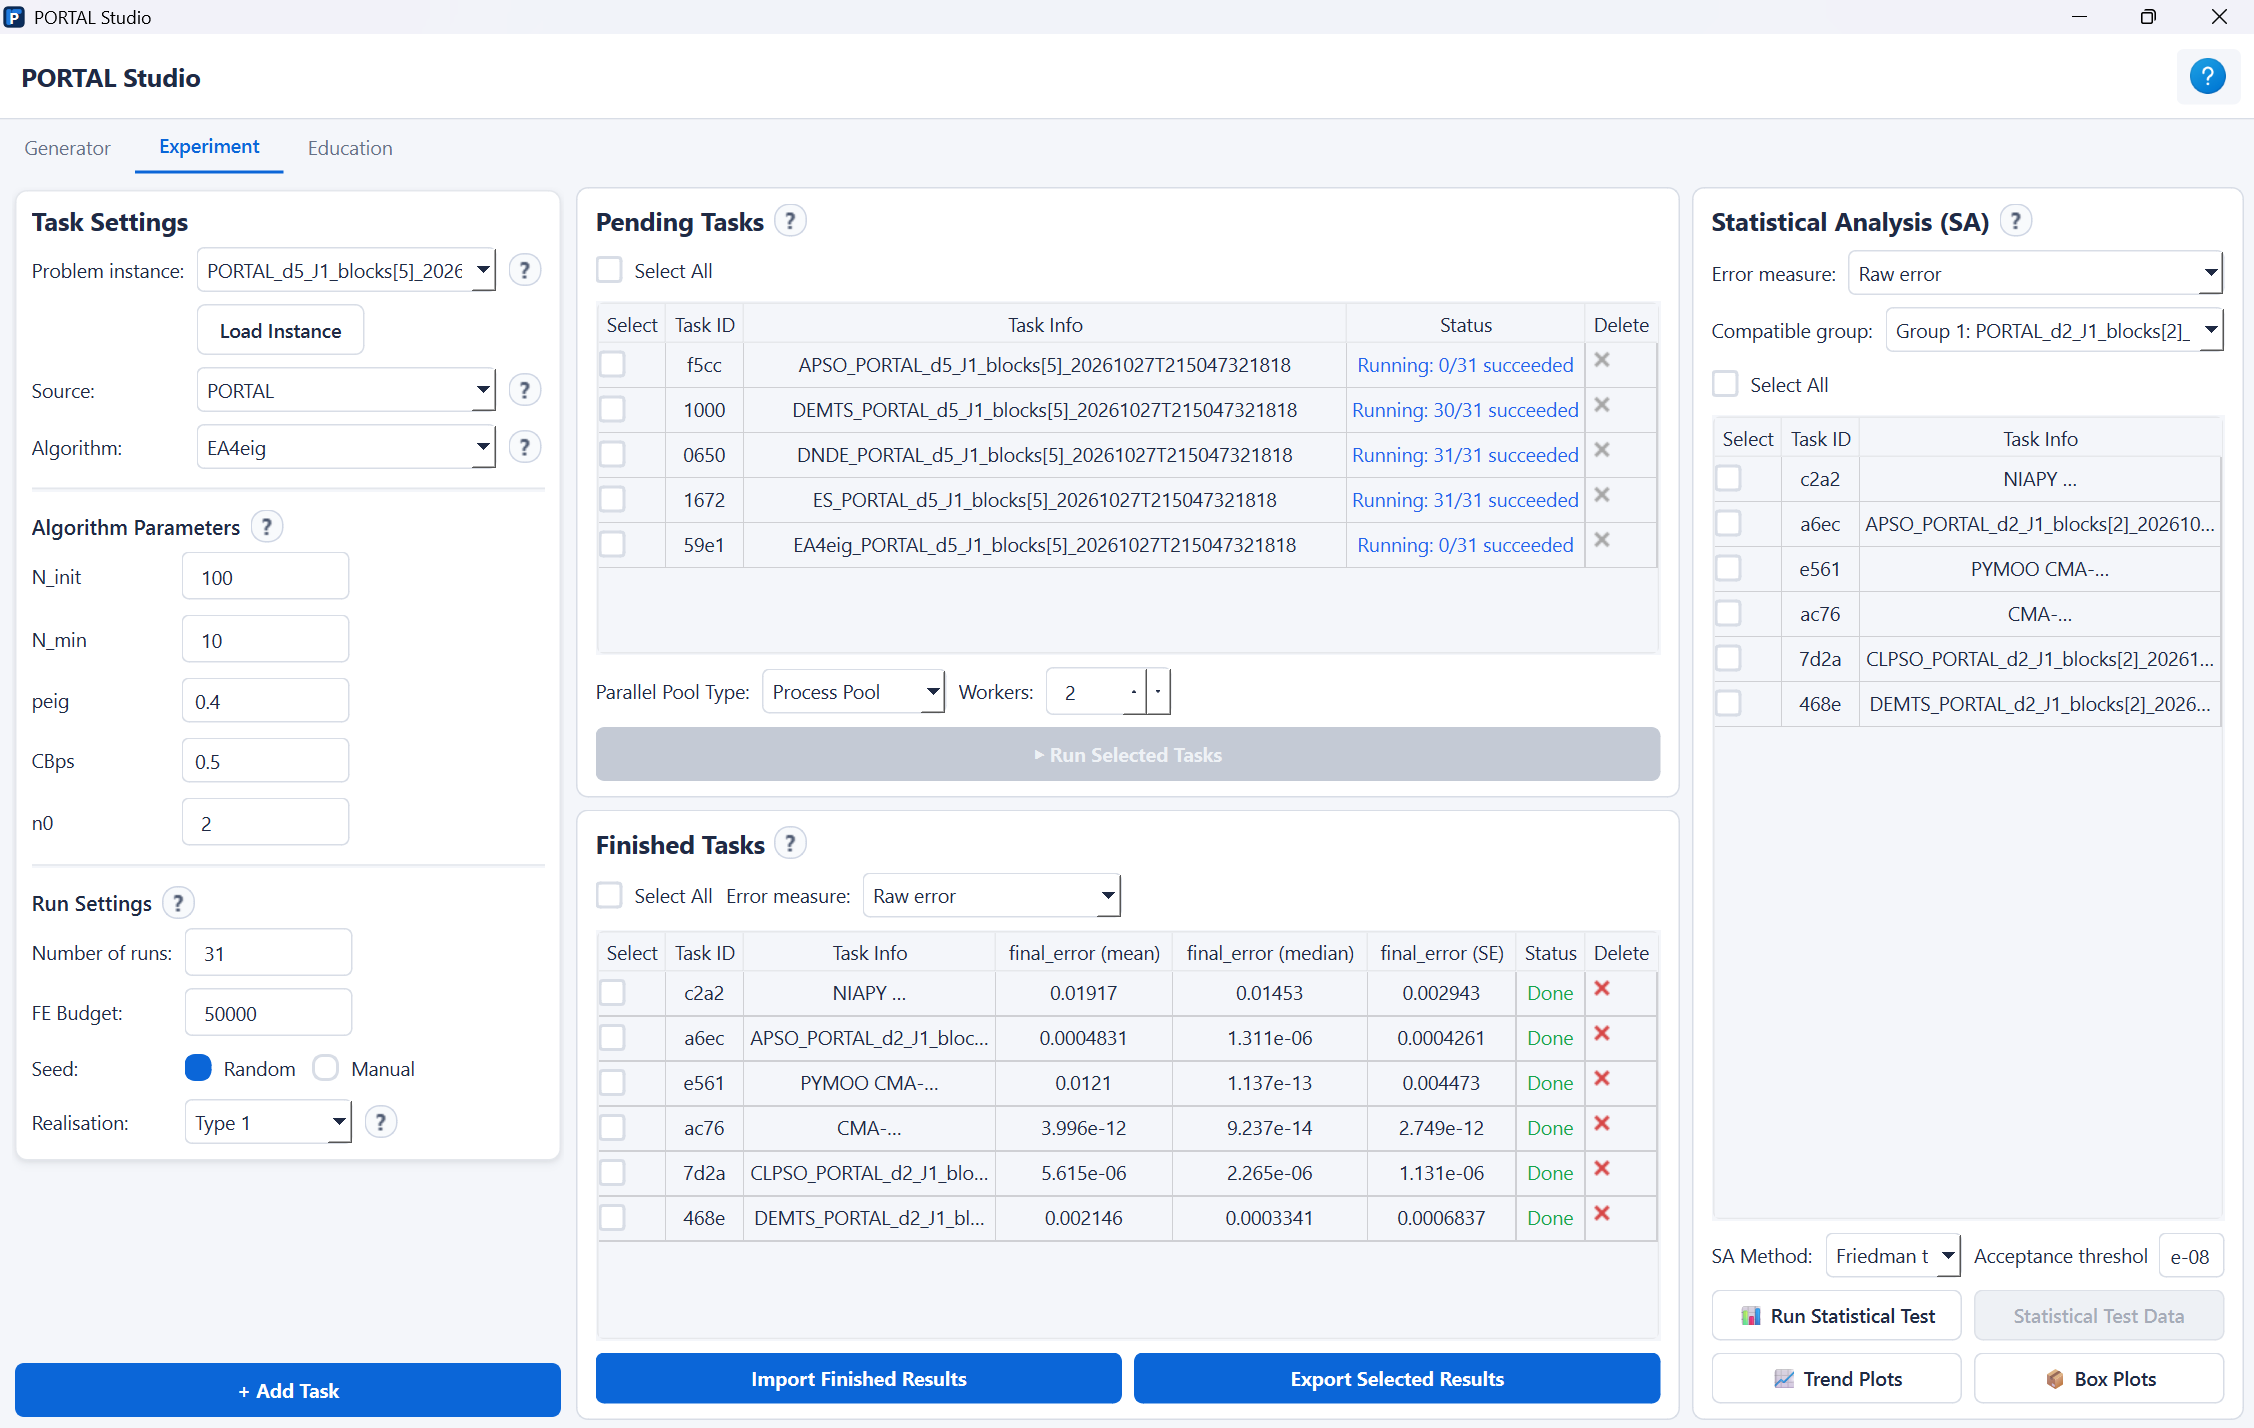
\includegraphics[width=\manualfigwidth]{6.png}
    \caption{Experiment workspace with Task Settings on the left, Pending and Finished Tasks in the middle, and Statistical Analysis on the right. The selected problem in Task Settings can differ from the compatible group selected for analysis.}
    \label{fig:manual:experimental-workspace}
\end{figure}

\subsection{Task Settings}
\label{ssec:manual:experimental-task-settings}

The \emph{Task Settings} panel defines an experiment task before it is added to the pending queue.

The \emph{Problem instance} row selects the PORTAL instance to be evaluated. Instances prepared in Generator automatically appear in this list when the Experiment workspace is opened. Use \emph{Load Instance} to load a saved PORTAL JSON file.

Algorithm selection uses two linked controls. First, \emph{Source} selects the implementation group: native PORTAL solvers or an integrated third-party package. The \emph{Algorithm} row then lists the optimisers available for that source, and the \emph{Algorithm Parameters} area updates to show the parameters exposed by the selected solver.

The \emph{Run Settings} area specifies the number of repeated runs, function-evaluation budget, algorithm seed policy, and realisation mode. \emph{Number of runs} gives the number of optimiser executions requested for the task, while \emph{FE Budget} sets the maximum objective-function evaluations per run.

The \emph{seed policy} controls the optimiser's random choices across runs, such as initial candidate solutions. \emph{Random} assigns seeds automatically. \emph{Manual} uses the entered \emph{Algorithm seed} for the first run and adds one for each subsequent run; for example, entering 42 gives seeds 42, 43, 44, and so on.

The initial run count is 31, with a range of 1--200. The FE budget initially follows $10{,}000d$, where $d$ is the selected instance dimension, within the allowed range of 100--10,000,000 evaluations. Once you edit the budget, changing the selected instance no longer updates it automatically. Choose and record settings appropriate to the study. Confirm that all requested runs completed successfully before treating a task as a complete repeated-run sample.

\subsubsection{Realisation Types}
\label{sssec:manual:experimental-realisations}

The \emph{Realisation} setting determines whether repeated runs use the stored problem or controlled variants of it. Type~0 keeps the problem unchanged for every run; Types~1 and~2 generate a variant for each run.

Type~1 changes component locations and shifts objective values while retaining shape and interaction settings. Type~2 also rearranges existing curvature, anisotropy, and signed transformation parameter values instead of drawing new values for those parameters. Either mode can change optimisation difficulty, since moving components within fixed search bounds can affect the search even when shape settings are unchanged. Landscape measurements may also change, including in response to objective shifts. Table~\ref{tab:manual:realisation-types} summarises the three modes.

\begin{table}[H]
\centering
\small
\caption{Realisation types available in the Experiment workspace. Type~3 augmentation is provided separately by the dataset runner.}
\label{tab:manual:realisation-types}
\begin{tabular}{@{}p{0.18\linewidth}p{0.72\linewidth}@{}}
\toprule
\textbf{Type} & \textbf{Experiment meaning} \\
\midrule
Type~0 & Evaluates the same stored landscape in every run. Different algorithm seeds can still produce different search behaviour. \\
Type~1 & Within each block, applies the same bounded translation to all component centres and the same shift to their objective-value offsets. Shape and interaction parameters, distances between centres, and differences between offsets are preserved within the block. \\
Type~2 & Within each block, attempts an orthogonal move of the centre configuration, followed by a bounded translation and a common objective-value offset shift. Existing signed parameter pairs are permuted and may swap directions; existing block weights are reassigned for multi-block recipes. Neutralisation factors are recalculated. \\
\bottomrule
\end{tabular}
\end{table}

To compare algorithms on equal terms, each should face the same problem variants. Studio therefore uses fixed realisation settings so that, for the same source problem and realisation type, corresponding runs evaluate matching variants.

Once the problem, algorithm, parameters, run settings, and realisation mode are configured, select \emph{+ Add Task} to add the task to \emph{Pending Tasks}.

\subsubsection{Package-Backed Algorithms}
\label{sssec:manual:experimental-package-algorithms}

PORTAL Studio supports optimisers from NiaPy~\cite{niapyjoss} and single-objective algorithms from PyMOO~\cite{blank2020pymoo}. Package-backed algorithms expose a small common set of GUI parameters, typically population size, so that they can be used consistently alongside PORTAL's native solvers. The corresponding Python package must be installed in the active environment before the algorithm can be run.

\subsection{Pending and Finished Tasks}
\label{ssec:manual:experimental-task-execution}

Tasks created in \emph{Task Settings} appear in \emph{Pending Tasks}. Tick one or more tasks, choose \emph{Process Pool} and the number of \emph{Workers}, or \emph{Serial (1 worker)}, then select \emph{Run Selected Tasks}. Each task expands into the requested repeated runs.

When a task completes, fails, or is cancelled, it moves to \emph{Finished Tasks}, which reports its summary and terminal state. Successfully completed tasks become available in Statistical Analysis. Deleting a finished task removes its row without deleting the on-disk bundle.

\paragraph{Saving and reopening finished results.}
Studio automatically saves run results under \path{results/raw_runs/batch_<timestamp>/}, relative to the folder from which Studio was launched. To keep selected finished tasks in a portable file for later analysis, tick their rows in \emph{Finished Tasks} and select \emph{Export Selected Results}. The ZIP archive preserves each task's algorithm settings, problem-source information, budget, seeds, realisation mode, status, recorded run errors, convergence checkpoints, and identities used for statistical pairing. Tasks retain their individual settings even when exported together. The archive also includes recorded run errors in \path{run_errors.csv} and convergence data in \path{convergence.csv}; both files can be opened in Excel.

Select \emph{Import Finished Results}, then choose the exported results ZIP file. The saved tasks are restored to \emph{Finished Tasks} without rerunning the experiments. Successfully completed tasks become available in Statistical Analysis.

\subsubsection{Experiment Output Measures}
\label{sssec:manual:experimental-output-measures}

In \emph{Finished Tasks}, the \emph{Error measure} selector offers the three measures summarised in Table~\ref{tab:manual:finished-task-fields}. Raw error is selected by default. For whichever measure is selected, Studio reports the \emph{mean}, \emph{median}, and \emph{standard error (SE)} across runs.

\begin{table}[H]
\centering
\small
\caption{Error measures available in Finished Tasks.}
\label{tab:manual:finished-task-fields}
\begin{tabular}{@{}p{0.27\linewidth}p{0.63\linewidth}@{}}
\toprule
\textbf{Measure} & \textbf{Meaning} \\
\midrule
\textbf{Raw error} & The absolute difference between the best objective value found and the evaluated instance's known optimum value, as defined in equation~\eqref{eq:manual:final-error}. \\
\textbf{Normalised error} & The raw error divided by the evaluated instance's reference scale. \\
\textbf{Reference-scale error (\%)} & The normalised error multiplied by 100. \\
\bottomrule
\end{tabular}
\end{table}

For run \(r\), the raw final error is
\begin{equation}
E_{\mathrm{final},r}=\left|B_{r,T}-F_r^\star\right|,
\label{eq:manual:final-error}
\end{equation}
where \(B_{r,T}\) is the best objective value found by the end of the evaluation budget \(T\), and \(F_r^\star\) is the known optimum value of the instance evaluated in that run.

For example, a run with raw error 6 and reference scale 120 has a normalised error of 0.05, equivalent to a reference-scale error of 5\%. Reference-scale percentages can exceed 100\%.

Normalised and percentage measures require enabled calibration for every component and a recorded reference scale. When these requirements are not met, \emph{Finished Tasks} displays a dash for those measures; raw results remain available. For blocks $b$ with positive weights $w_b$, component offsets $\beta_{b,k}$, and declared calibration rises $\Delta_{b,k}$, the nominal scale is
\begin{align}
S_{\mathrm{ref}}=\sum_b w_b\left[\max_k(\beta_{b,k}+\Delta_{b,k})-\min_k\beta_{b,k}\right].
\end{align}
It describes declared reference levels, not the attained objective range or problem difficulty. The value is computed from the concrete instance used in each run.

\subsection{Statistical Analysis}
\label{ssec:manual:experimental-statistical-analysis}

The \emph{Statistical Analysis (SA)} panel compares results from finished tasks. It provides statistical tests of final errors, convergence plots, and final-error distributions. Start by choosing the error measure and a group of compatible tasks, then select the tasks to analyse.

\paragraph{Choosing a measure and group.}
Select \emph{Raw error}, \emph{Normalised error}, or \emph{Reference-scale error (\%)} from \emph{Error measure}. This selection applies to both tests and plots. Normalised and percentage measures require a valid recorded reference scale for every run; tasks without one are excluded from those measures but can remain available under Raw error.

The \emph{Compatible group} menu updates automatically for the selected measure. Each group contains successfully completed tasks with valid run data and matching:
\begin{itemize}
    \item \textbf{Recorded problem identities:} corresponding runs evaluated the same source problem and concrete problem variants.
    \item \textbf{Realisation type:} the tasks used the same realisation mode.
    \item \textbf{Evaluation budget and run count:} the tasks used the same FE budget and requested number of runs.
\end{itemize}
Different algorithms, algorithm parameters, and algorithm seeds are allowed within a group. For example, PSO and DE can be compared when their corresponding runs evaluate matching Type~1 variants under the same budget.

Choose a group, then tick the task rows to include, or use \emph{Select All}. Tasks with different problem identities or trial settings appear in separate groups. Changing the error measure rebuilds the groups and clears the selected rows and previous test results.

\paragraph{Running a statistical test.}
Each selected task must contain at least two completed runs. Comparisons are paired by run index: run~1 of one task is compared with run~1 of the other tasks on the matching problem, and likewise for subsequent runs. Choose the test from \emph{SA Method}:
\begin{itemize}
    \item \textbf{Friedman test:} compares at least three selected tasks using their per-run final errors in the chosen error measure. If the overall test is significant, Studio reports pairwise Wilcoxon signed-rank comparisons with Holm correction.
    \item \textbf{Wilcoxon signed-rank:} select two tasks for a direct paired comparison. If more tasks are selected, Studio reports all pairwise comparisons with Holm correction.
\end{itemize}
Select \emph{Run Statistical Test}, then \emph{Statistical Test Data} to view the result tables. Studio checks the recorded data for validity and compatible pairing before testing. The significance level is fixed at $\alpha=0.05$; pairwise significance is determined from the Holm-adjusted $p$-values. An \texttt{n/a} entry means that a comparison is undefined, for example because its paired error samples are identical.

\paragraph{Viewing convergence and final errors.}
Use \emph{Trend Plots} or \emph{Box Plots} for the selected tasks; a statistical test is not required first. Trend plots show the mean best-so-far error across runs, with a band of one standard error on either side, as illustrated in Figure~\ref{fig:manual:sa-example-trend}. Box plots show the distribution of final errors. Both use the selected error measure, and a task with one completed run can be plotted.

The \emph{Acceptance threshold} marks a target error as a reference line on the trend plot. Enter it in the selected measure's units; changing the measure clears the previous threshold. This target is separate from the statistical significance level. Use \emph{Export} in a plot window to save PNG, PDF, or SVG.

\begin{figure}[H]
    \centering
    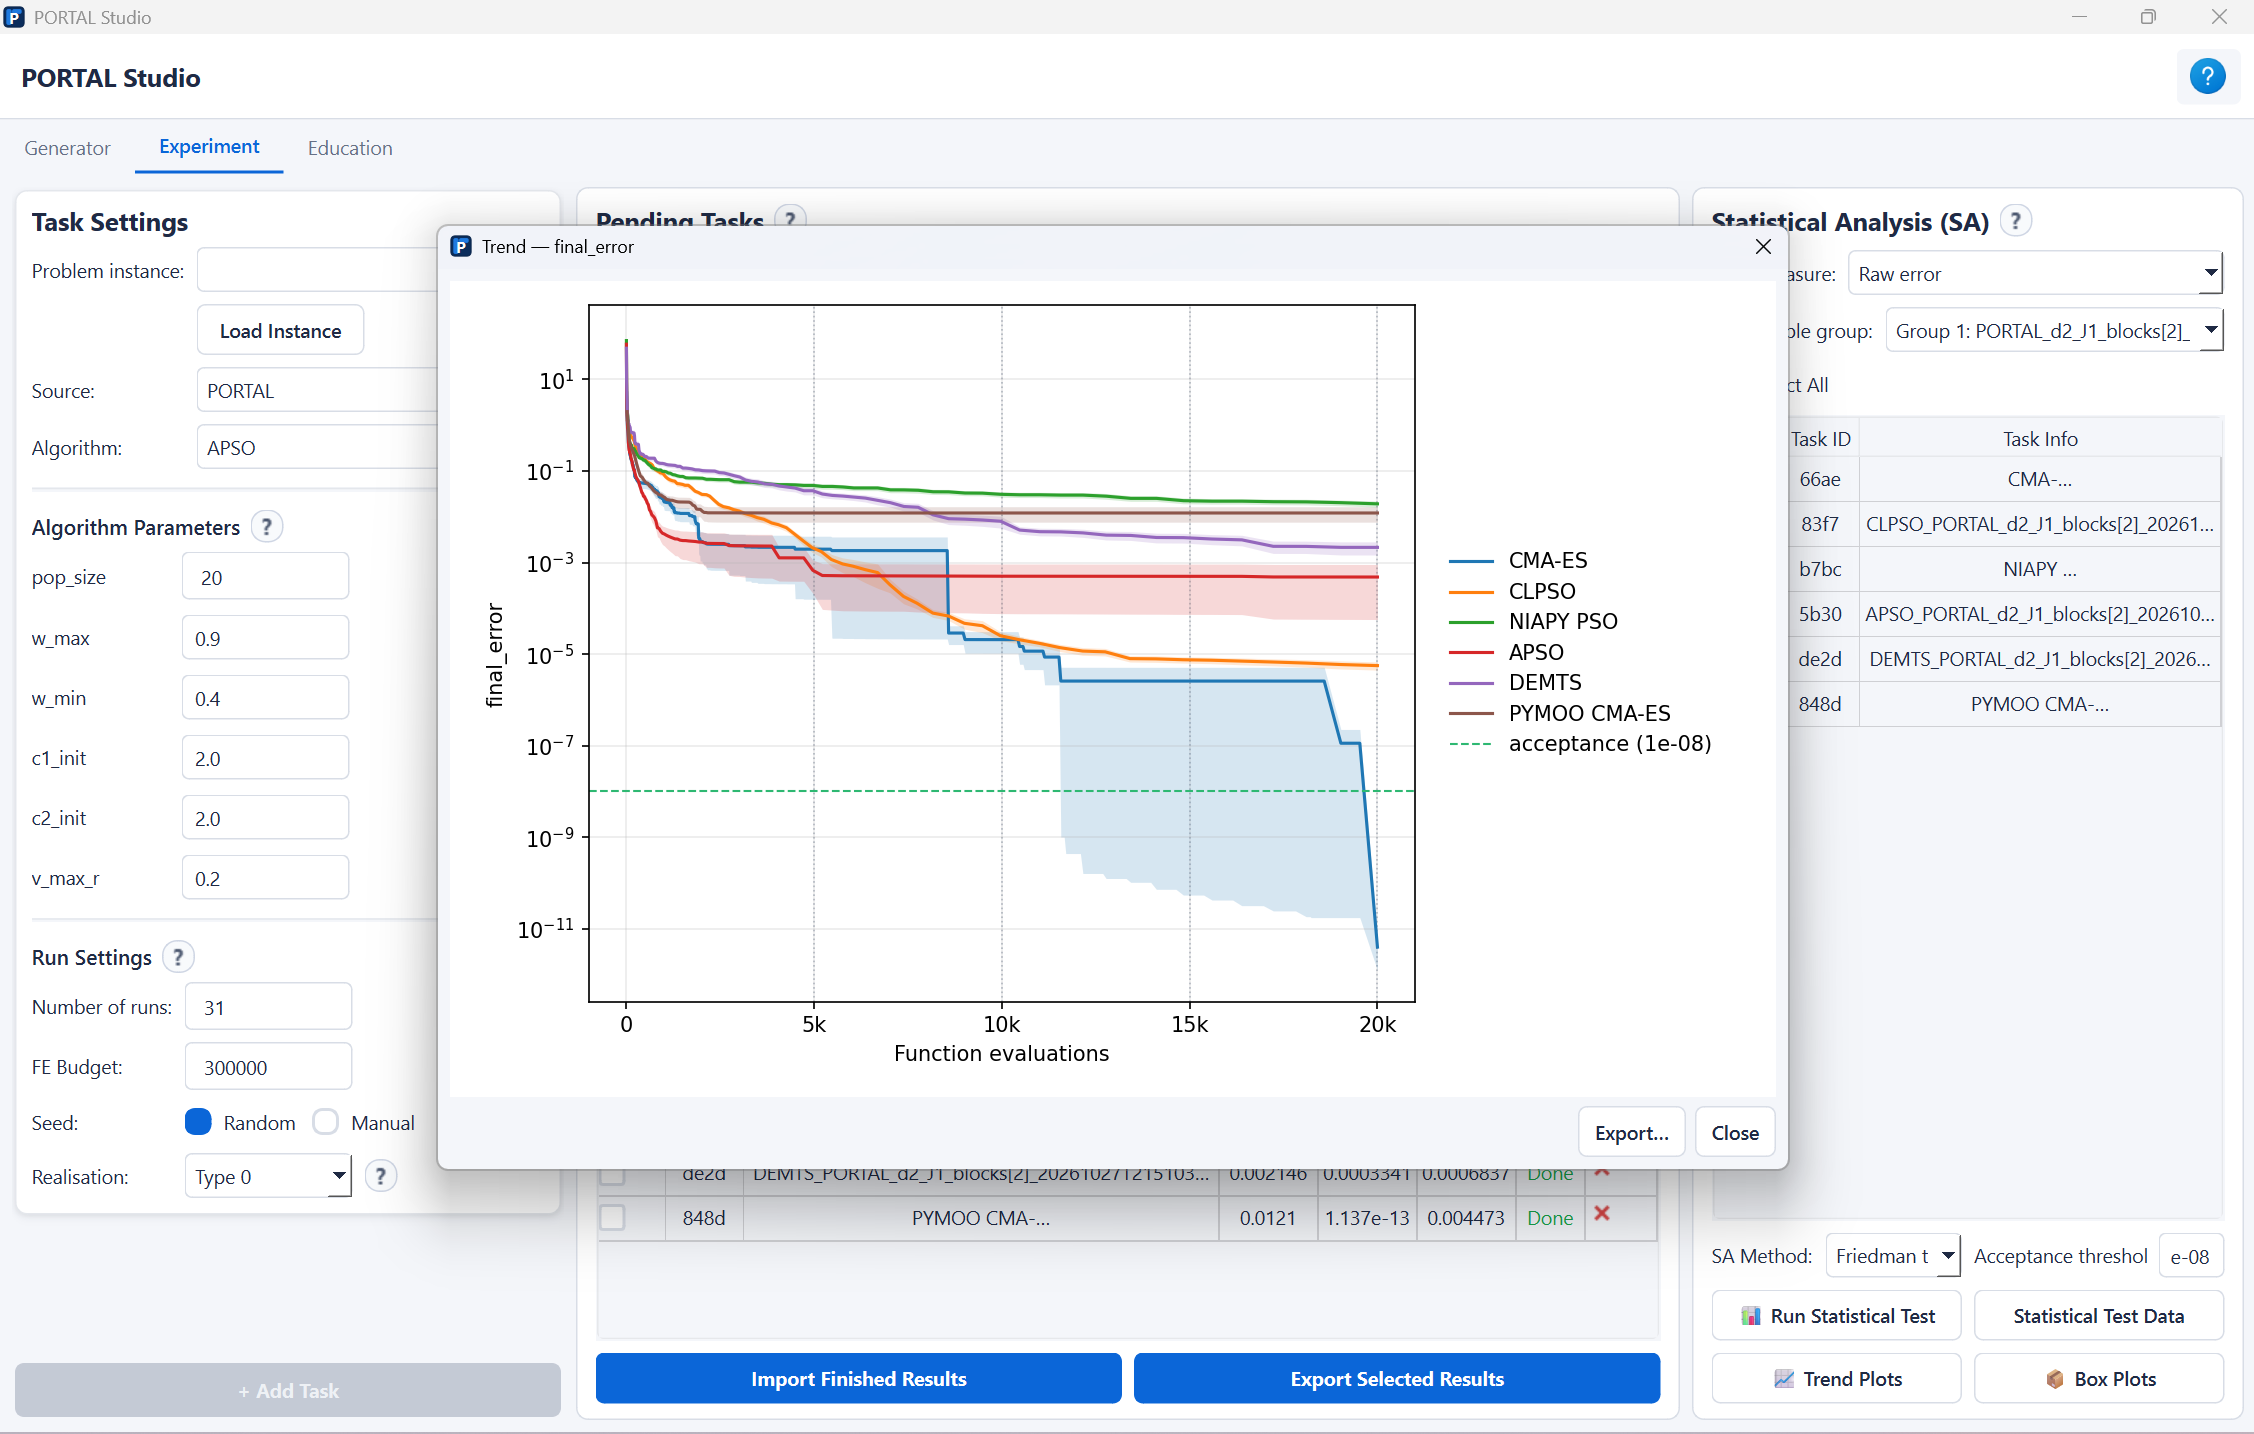
\includegraphics[width=\manualfigwidth]{11.png}
    \caption{Raw-error convergence for six algorithms on a two-dimensional, single-block source problem, using 31 Type~1 runs per task and a budget of 20,000 function evaluations. Curves show across-run means with bands of one standard error. The error axis uses a logarithmic scale; the dashed green line marks the acceptance threshold of $10^{-8}$.}
    \label{fig:manual:sa-example-trend}
\end{figure}

\FloatBarrier
\section{Education Workspace}
\label{sec:manual:educational}

The \textbf{Education} workspace provides an interactive two-dimensional environment for exploring PORTAL landscape construction and optimiser behaviour. Users can modify component parameters, observe their effects on the landscape, and examine how optimisers move and converge during search.

The workspace contains two connected views: \textbf{2-D Authoring}, where components and landscapes are constructed and visualised, and \textbf{Benchmarking}, where the resulting landscapes are used for optimiser demonstrations and comparison.

\subsection{2-D Authoring View}
\label{ssec:manual:educational-authoring}

The \textbf{2-D Authoring} view (Figure~\ref{fig:manual:educational-authoring}) lets users build landscapes in two variables and inspect how component settings affect their shape. Parameters are entered directly for each coordinate, and rotation angles use degrees.

\paragraph{Create and edit an instance.}
Select \textbf{+ Add Instance}, then use the instance row's plus control to open a component editor. Enter its parameters and select \textbf{+ Add Component}. Repeat to add more components. To edit an existing component, select its row, change the settings, and select \textbf{Apply Changes}.

\paragraph{Inspect the landscape.}
Select a component to view it individually, or select the instance to view the combined landscape. \textbf{Current Landscape} provides surface and contour plots; \textbf{Visualize Components} and \textbf{Visualize Instances} provide side-by-side comparisons.

\begin{figure}[!t]
    \centering
    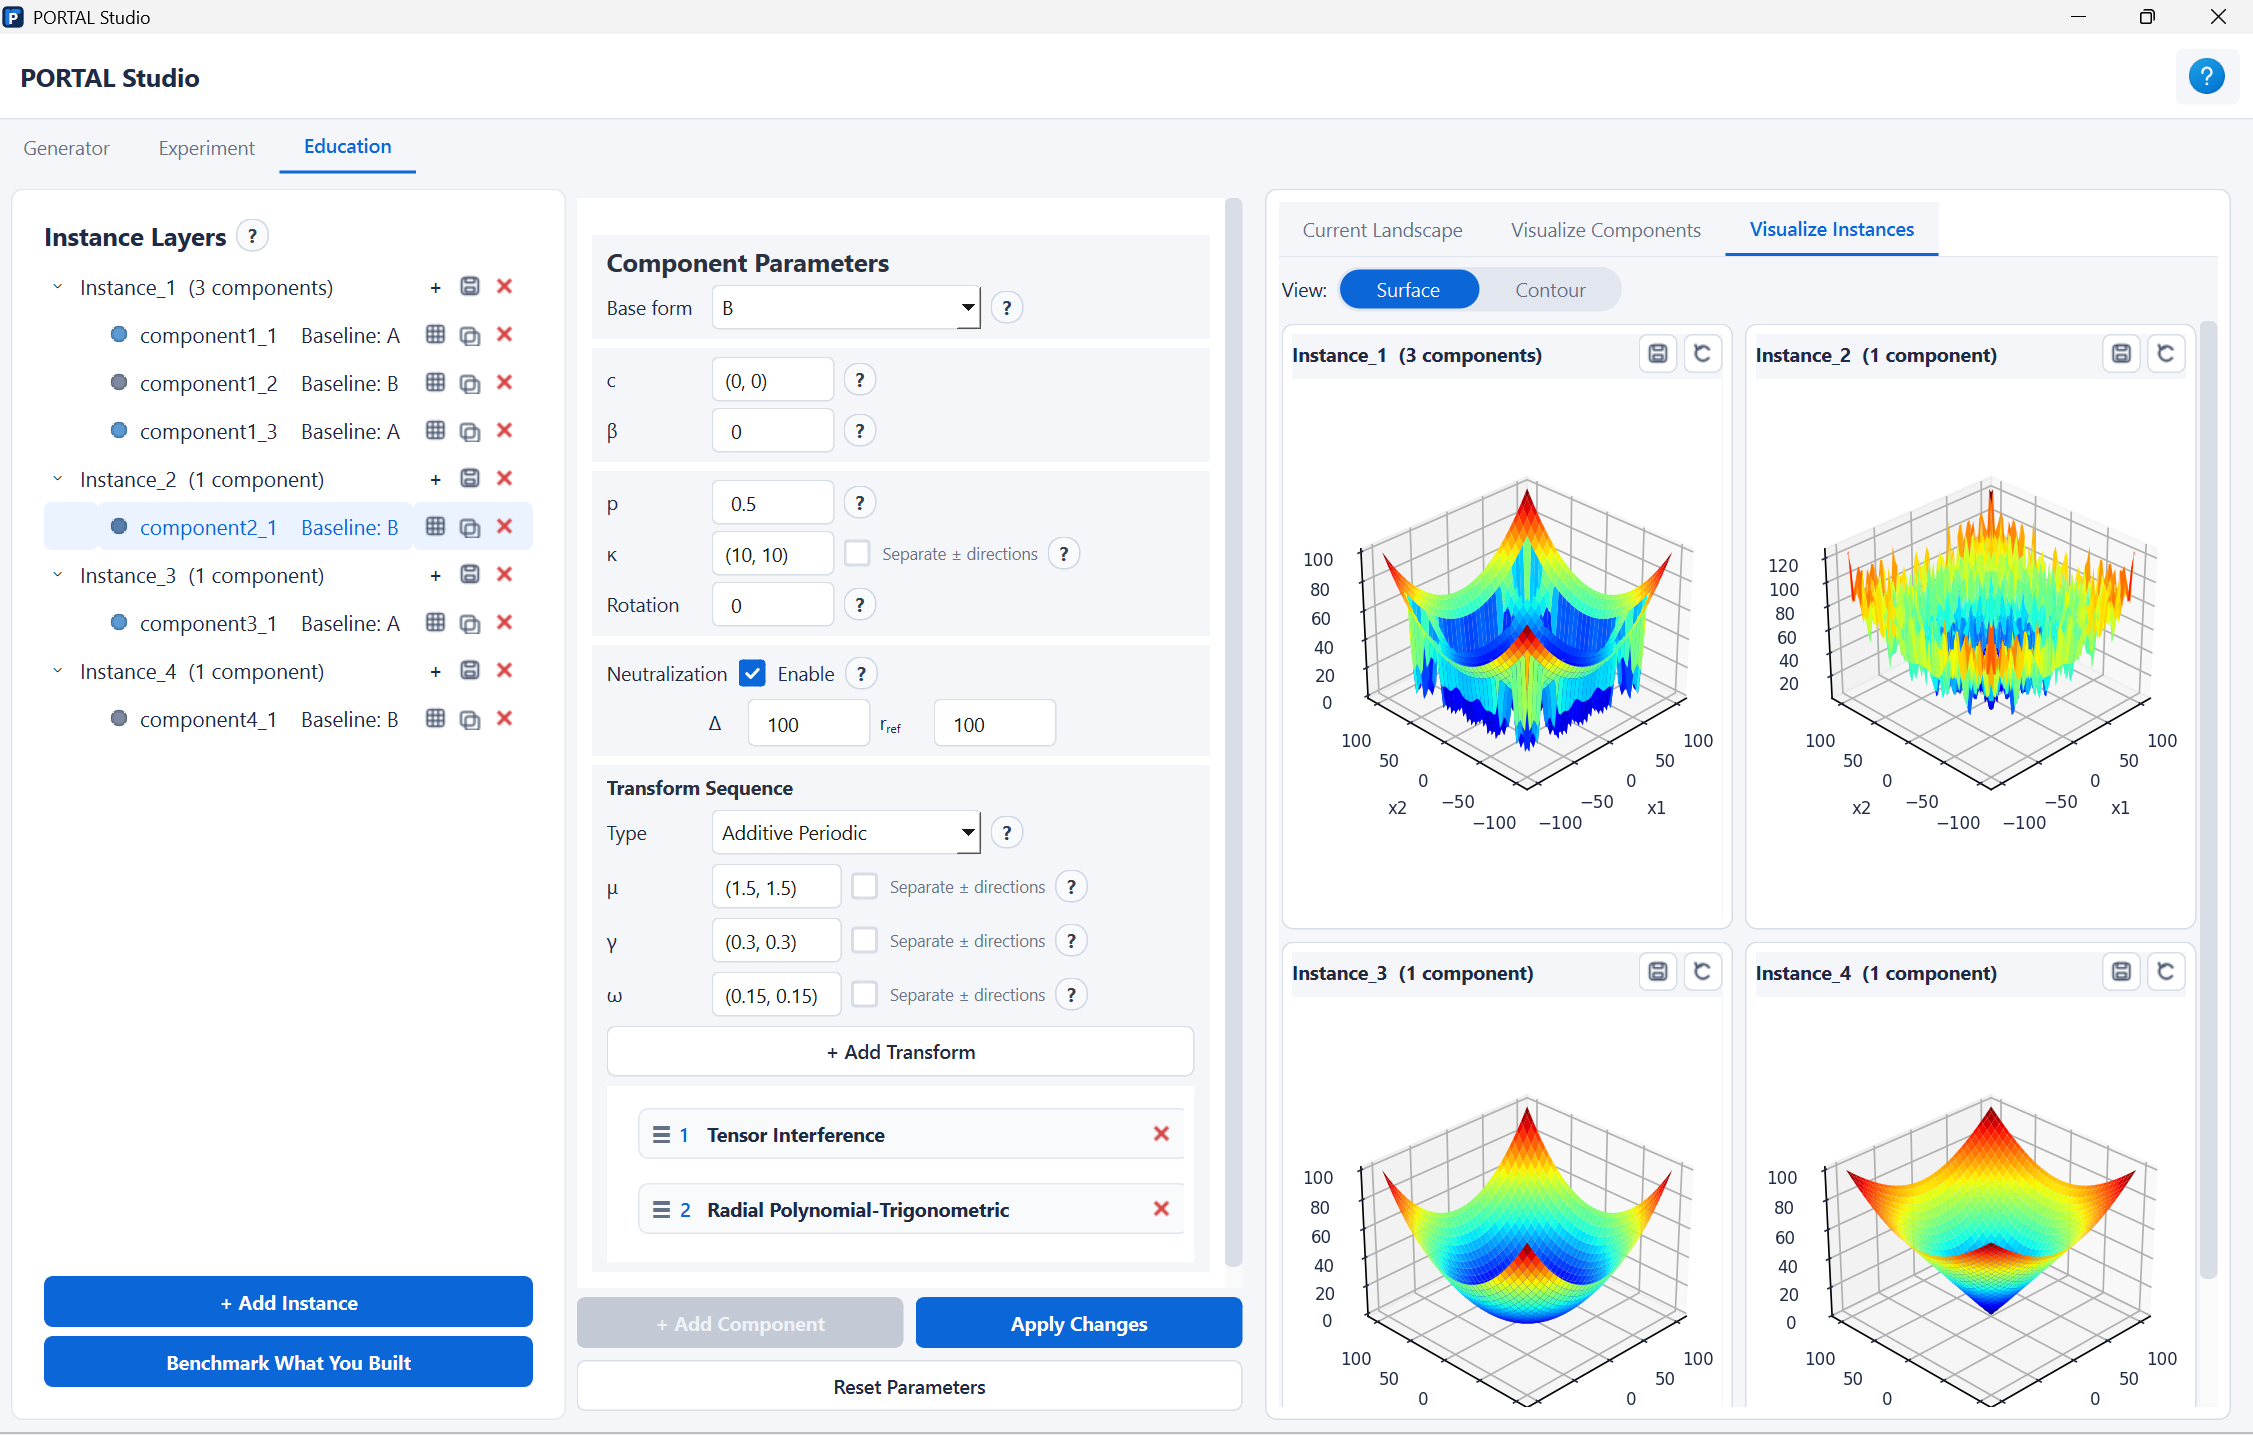
\includegraphics[width=\manualfigwidth]{7.png}
    \caption{Education's 2-D Authoring view. Instance Layers appear on the left, component settings in the middle, and the \emph{Visualize Instances} surface comparison on the right.}
    \label{fig:manual:educational-authoring}
\end{figure}

\paragraph{Add transformations.}
Choose a transformation \emph{Type}, configure its parameters, and select \emph{+ Add Transform}. Drag sequence rows to reorder them or use their cross controls to remove them. Save sequence changes with \emph{Apply Changes} for an existing component or \emph{+ Add Component} for a new one.

To edit a transformation, select its row, change its parameters, and select \emph{Apply Changes}. For an existing component, select \emph{Apply Changes} again to save the updated component. To explore transformation order, clone a component and reorder its transformations while keeping the other settings unchanged. Use \emph{Visualize Components} to compare their surfaces or contours.

\paragraph{Save your work.}
Use the instance row's \emph{Save this instance as JSON} icon to save the problem for later use in Experiment. Plot save icons export individual figures as PDF.

\subsection{Benchmarking View}
\label{ssec:manual:educational-benchmarking}

The \textbf{Benchmarking} view shows how an optimiser searches an authored landscape and how its error changes during the run. Select \textbf{Benchmark What You Built} to open this view; use the toolbar back arrow to return to \textbf{2-D Authoring}.

\paragraph{Run an optimiser.}
Select the problem instance, choose a \emph{Source} and \emph{Algorithm}, and configure the algorithm parameters. These controls work as in Experiment (Section~\ref{ssec:manual:experimental-task-settings}). Set \emph{Budget (FE)} and select \emph{Run}. The running dialog's \emph{Cancel} control requests cancellation during computation.

The initial budget is 20,000 evaluations for a two-dimensional problem, with an allowed range of 10--1,000,000. Education uses algorithm seed 42. The \emph{Acceptance rate} field sets the target absolute error shown as a reference line on the convergence plot; its default is $10^{-8}$.

\paragraph{Compare two setups.}
Enable \textbf{Comparison mode} to display Setup~A and Setup~B. Choose an instance, source, algorithm, and parameters for each setup, then select \emph{Run}. Both setups use the same budget and acceptance threshold. Their recorded runs are replayed together at matching evaluation counts, as illustrated in Figure~\ref{fig:manual:educational-benchmarking}. Use Experiment for comparisons over repeated runs and statistical analysis.

\paragraph{Replay the results.}
Playback starts automatically after computation finishes. Search positions appear over the landscape, while the convergence plot shows the best-so-far absolute error relative to the evaluated instance's known optimum. Use \emph{Play}/\emph{Pause} to control playback, \emph{Reset} to return to the start, \emph{Speed} to change the playback rate, or drag the FE slider to inspect a recorded evaluation. These controls replay the recorded run without running the optimiser again.

Surface and contour plots use a finite sampling grid, so very narrow landscape features may not be visible.

\begin{figure}[H]
    \centering
    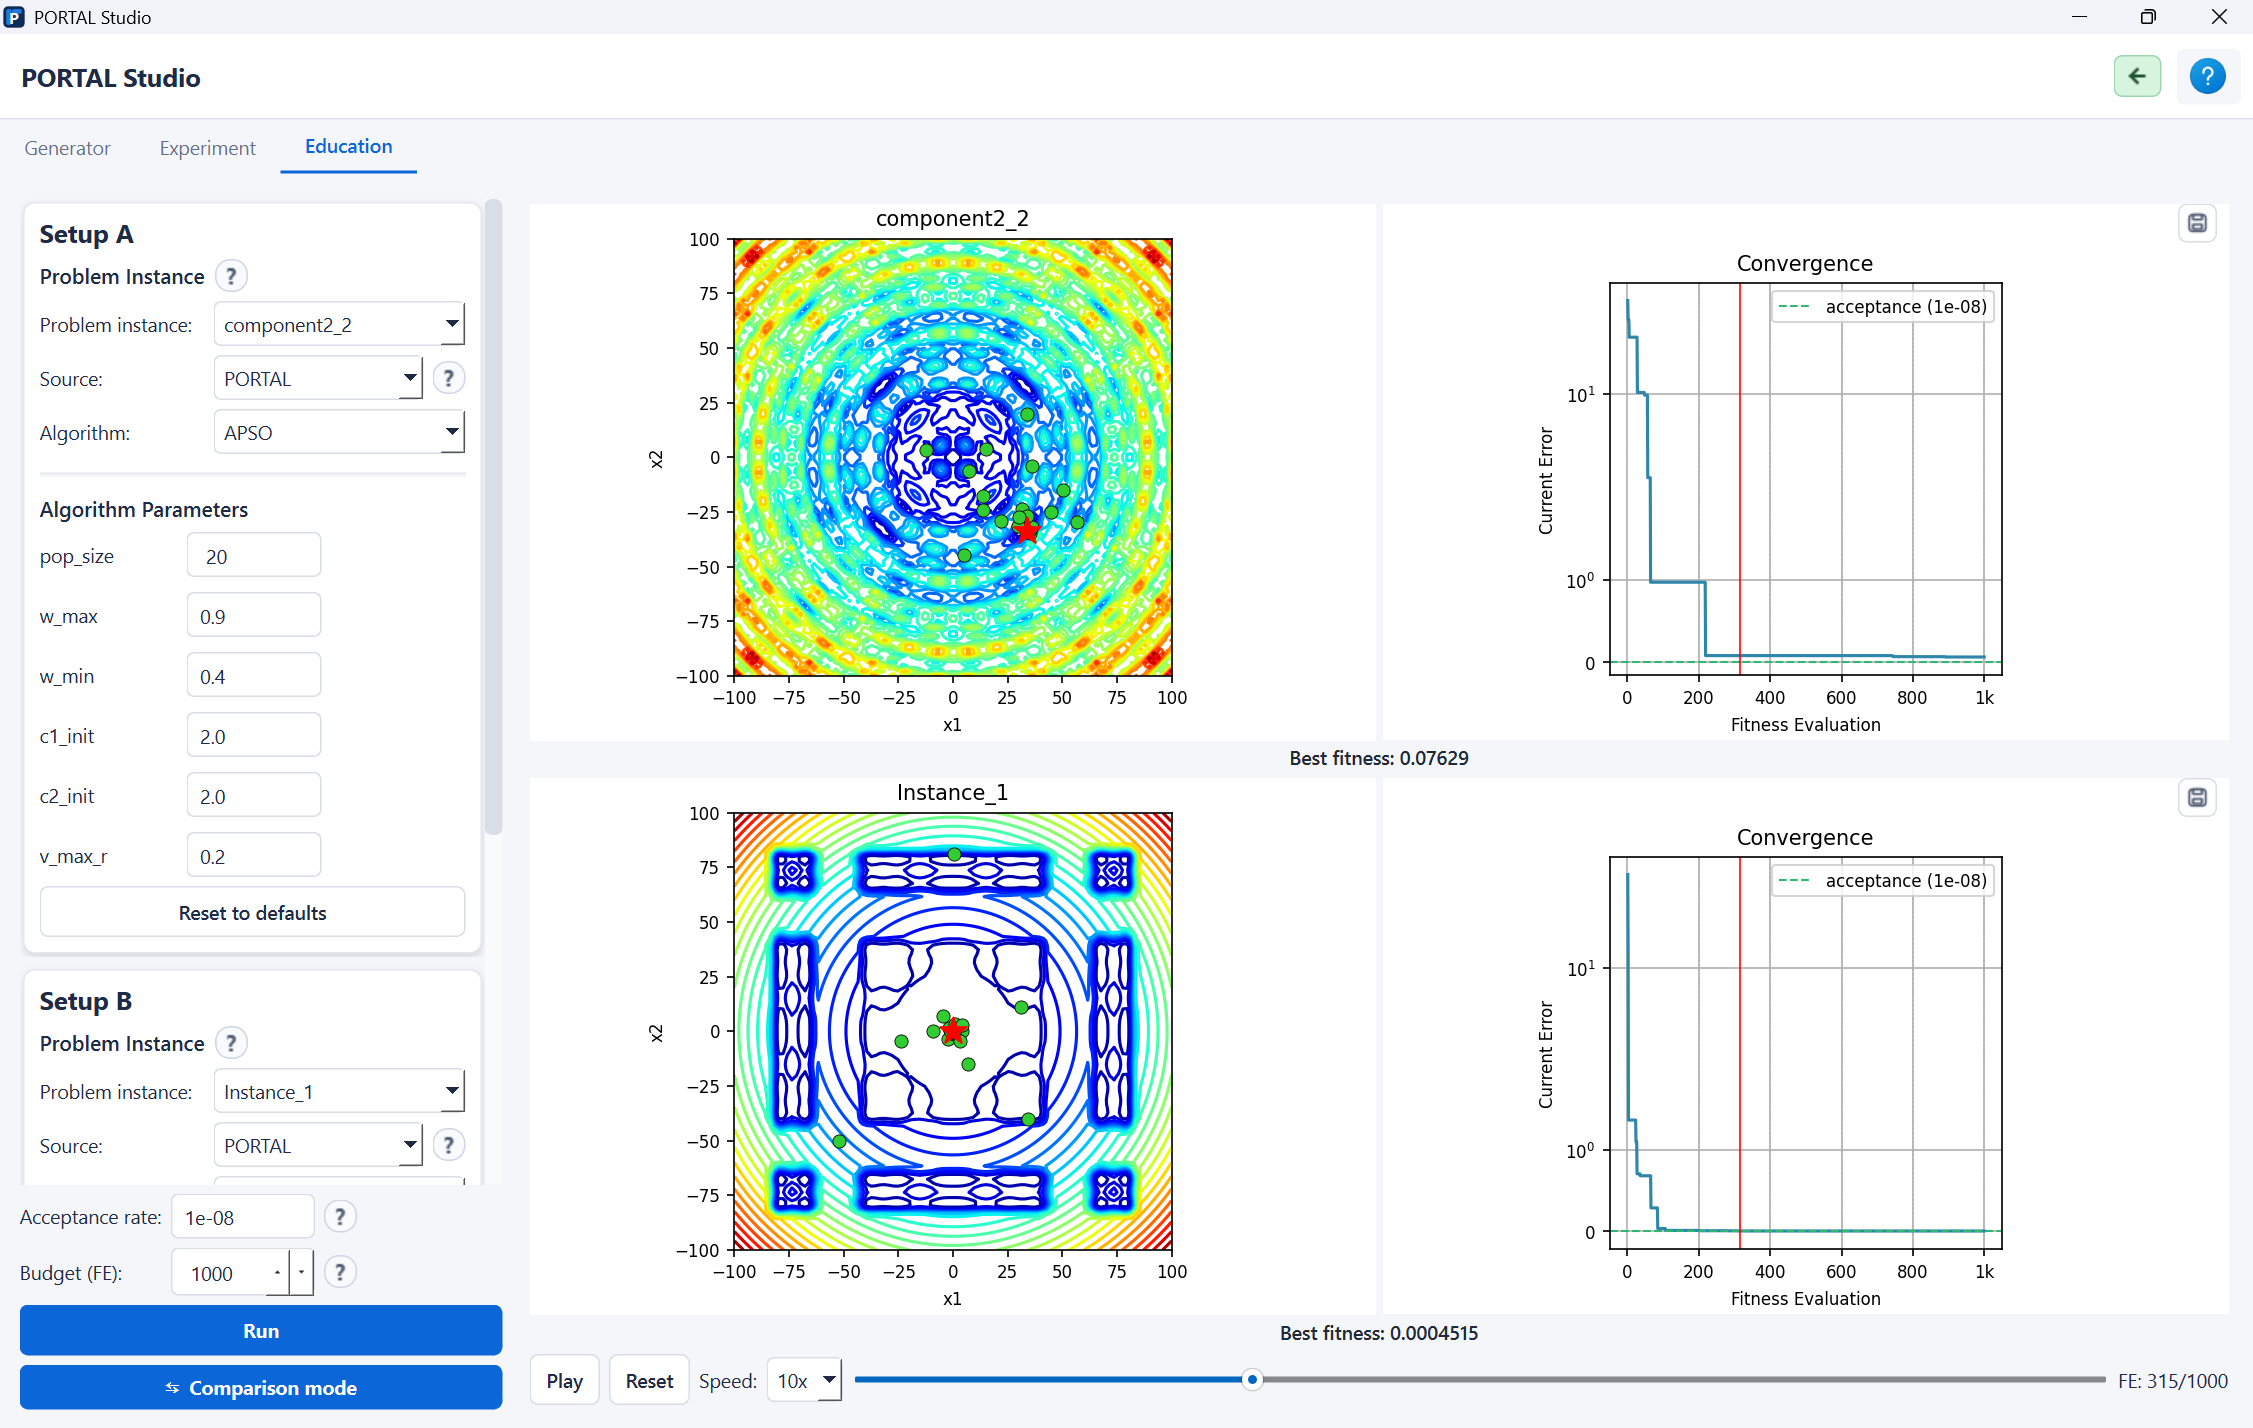
\includegraphics[width=\manualfigwidth]{8.png}
    \caption{Education Benchmarking in comparison mode. The two setups show search positions over contour plots and their best-so-far error curves. Playback is paused at evaluation 315 of a 1,000 FE budget; dashed green lines mark the acceptance threshold of $10^{-8}$.}
    \label{fig:manual:educational-benchmarking}
\end{figure}

\FloatBarrier
\section{Adding a Solver to the GUI}
\label{sssec:manual:experimental-solver-gui}

You can add your own optimisation algorithm to Studio by creating a Python wrapper in the repository's \path{algorithms/} directory. Studio discovers these wrappers at startup and makes them available in Experiment and Education Benchmarking.

\paragraph{1. Create the wrapper.}
Create a file such as \path{algorithms/MySolver.py}. Define a class that inherits from \texttt{BaseAlgorithm} and implements \texttt{run(problem)}. The \texttt{problem} object provides the dimension, search bounds, evaluation methods, and budget check.

\begin{samepage}
The following minimal example samples candidates uniformly within the search bounds. Replace its sampling step with your algorithm's search procedure.

\begin{verbatim}
"""MySolver -- Minimal example of a PORTAL solver wrapper."""

import numpy as np
from base_algorithm import BaseAlgorithm


class MySolver(BaseAlgorithm):
    def __init__(self):
        super().__init__(name="MySolver")

    def run(self, problem):
        while not problem.is_done():
            x = np.random.uniform(
                problem.lb, problem.ub, size=problem.d
            )
            value = problem.evaluate(x)
            # Use value to update your algorithm's search state.

        return self._make_result(problem)
\end{verbatim}
\end{samepage}

Evaluate every candidate through \texttt{problem.evaluate(x)}, or use \texttt{problem.evaluate\_batch(X)} for batches of candidates. These methods count function evaluations and update the recorded best solution. Check \texttt{problem.is\_done()} before requesting further evaluations, and return \texttt{self.\_make\_result(problem)} when the run ends.

\paragraph{2. Expose the algorithm's parameters.}
Add configurable parameters to the class constructor, give them suitable defaults and type annotations, and store them for use in \texttt{run}. For example, a population-based solver might define:

\begin{verbatim}
def __init__(self, pop_size: int = 30):
    super().__init__(name="MySolver")
    self.pop_size = pop_size
\end{verbatim}

Studio reads the constructor arguments to create the \textbf{Algorithm Parameters} controls. To specify input ranges, step sizes, tooltips, or categorical choices, add an entry under the solver's displayed name in \texttt{PARAM\_OVERRIDES} in \path{portal_studio/algorithms/solver_params.py}. Existing entries provide examples.

\paragraph{3. Restart Studio and select the solver.}
Install any dependencies required by your wrapper in the Python environment used to launch Studio, then restart Studio. Select \textbf{PORTAL} as the algorithm \textbf{Source} and choose your solver from the \textbf{Algorithm} list. By default, the displayed name comes from the wrapper's filename: \texttt{MySolver.py} appears as \textbf{MySolver}.

If the solver does not appear, check that the file imports successfully and defines its own \texttt{BaseAlgorithm} subclass with a \texttt{run} method. Studio skips wrappers that fail to import.

\paragraph{4. Check the integration.}
Start with a small evaluation budget and confirm that the solver runs, respects the budget, and produces results and a convergence plot. Then check that changing its GUI parameters affects the settings used by the algorithm. The existing wrappers in \path{algorithms/} provide examples of complete solver implementations.

\clearpage
\bibliography{manual_references}
\bibliographystyle{IEEEtran}

\end{document}
